%% LyX 2.0.5 created this file.  For more info, see http://www.lyx.org/.
%% Do not edit unless you really know what you are doing.
\documentclass[british,english]{article}
\usepackage[T1]{fontenc}
\usepackage[latin9]{inputenc}
\usepackage{listings}
\usepackage{geometry}
\geometry{verbose,tmargin=3cm,bmargin=3cm,lmargin=3cm,rmargin=3cm}
\usepackage{array}
\usepackage{fancybox}
\usepackage{calc}
\usepackage{bbding}
\usepackage{graphicx}

\makeatletter

%%%%%%%%%%%%%%%%%%%%%%%%%%%%%% LyX specific LaTeX commands.
%% Because html converters don't know tabularnewline
\providecommand{\tabularnewline}{\\}

%%%%%%%%%%%%%%%%%%%%%%%%%%%%%% User specified LaTeX commands.
\usepackage{verbatim}
%\usepackage{xcolor}
\usepackage{listings}
\lstdefinestyle{Bash}
{language=bash,
keywordstyle=\color{blue},
basicstyle=\ttfamily,
morekeywords={moosuser@machine},
alsoletter={:~$},
morekeywords=[2]{moosuser@machine:},
keywordstyle=[2]{\color{red}},
literate={\$}{{\textcolor{red}{\$}}}1 
         {:}{{\textcolor{red}{:}}}1
         {~}{{\textcolor{red}{\textasciitilde}}}1,
}

\usepackage[usenames,dvipsnames]{xcolor}

\usepackage{listings}

\lstset{
tabsize=4,
language=matlab,
        basicstyle=\small,
        %upquote=true,
        aboveskip={1.5\baselineskip},
        columns=fixed,
        showstringspaces=false,
        extendedchars=true,
        breaklines=true,
        prebreak = \raisebox{0ex}[0ex][0ex]{\ensuremath{\hookleftarrow}},
frame=single,
        showtabs=false,
        showspaces=false,
        showstringspaces=false,
        identifierstyle=\ttfamily,
        keywordstyle=\color[rgb]{0,0,1},
        commentstyle=\color[rgb]{0.133,0.545,0.133},
        stringstyle=\color[rgb]{0.627,0.126,0.941},
language=c++
}

\@ifundefined{showcaptionsetup}{}{%
 \PassOptionsToPackage{caption=false}{subfig}}
\usepackage{subfig}
\makeatother

\usepackage{babel}
\begin{document}

\title{A Guide to using MOOS-V10 Communications }


\author{Paul Newman, University of Oxford}

\maketitle
\begin{center}

\includegraphics[width=3cm]{images/MOOSV-10-256}
\par\end{center}

\begin{center}
\vspace{2cm}....ten years on
\par\end{center}

\newpage{}

\tableofcontents{}

\newpage{}


\section{Headlines - What's New?}

MOOS Version 10 is a major new release of MOOS. It comes just over
10 years after MOOS was first written and it incorporates many changes
that improve its performance and answer to requests made by the user
community. This document sets out the features, changes and their
implications on users of the communications API of MOOS. 


\subsection*{Functional Headlines}
\begin{itemize}
\item \textbf{Low latency} Asynchronous communications are now supported
via an upgraded \texttt{MOOSDB} and a new kind of communications client
object \texttt{MOOSAsyncCommClient.} This allows data to be pushed
to clients by the \texttt{MOOSDB} rather than clients having to fetch
messages which match their subscriptions when the call into the \texttt{MOOSDB. }This
affords a drastically decreased latency between data being published
and clients receiving it. Latencies are routinely sub-millisecond
now.
\item \textbf{Multithreaded design} The \texttt{MOOSDB} now offers improved
resilience when working with clients which reside at the end of a
high latency or low bandwidth link. Each client is now furnished with
its own thread within the DB which allows each client to take as long
as it needs to complete and \texttt{read} or \texttt{write }without
holding up the interactions of other clients. This behaviour can be
disabled from the command line in which case the behaviour of the
DB reverts to pre V10 behaviour.
\item \textbf{Wildcard subscriptions} The \texttt{MOOS }communications API
now supports wildcard subscriptions whereby clients can subscribe
to variable which match variable name patterns and also source name
patterns. For example a client could register for ``{*}:{*}'' meaning
all variables from all sources or ``J{*}:{*}K'' meaning any variable
beginning with ``J'' from a process ending in ``K'' 
\item \textbf{Configurable behaviour} in the way CMOOSApp handles mail.
You can have mail handled pretty much as soon as it comes in. If you
are using the low level comms object \texttt{MOOSAsyncCommClient}
you can have a call back handled the instant mail arrives.
\item \textbf{Standard Command Line Switches} All MOOS applications can
with a trivial code change be configured to handle and interpret standard
command line parameters. Additionally, a tool is provided to ease
parsing command line options. CMOOSApp has new hooks to support and
encourage the writing of user help and example configurations which
can be printed to stdio.
\item \textbf{A new build system }is provided which via CMake make linking
against MOOS (and the right version) easy.
\item \textbf{New testing} command line programs which can easily be used
to test MOOS communications
\item \textbf{Live diagnostics} from the MOOSDB are avaiable over udp
\end{itemize}

\subsection*{Structural Headlines}
\begin{itemize}
\item \textbf{Fission into smaller, neater delineated code trees:} The communication
layer, utility applications (like \texttt{pLogger}), and graphical
tools all now live in \foreignlanguage{british}{separate} projects.
For example, it is now possible to download only the communications
layer and work just with that.
\item \textbf{A single core library:} There is now just one core library
\texttt{libMOOS} which is an amalgamation of what was previously \texttt{MOOSGenLib}
and \texttt{MOOSLib}
\item \textbf{A }\foreignlanguage{british}{\textbf{rationalised}}\textbf{
header file structure:} The header structure for commonly used files
has changed to reflect this (but a backwards compatibility mode is
provided so users can in the first instance carry on as if this is
not the case)
\end{itemize}

\section{Structural Changes}


\subsection{Separate Projects}

Pre version 10, the MOOS project was an ugly mash-up of source code
which covered a strange span of functionality. This belied its Maritime
roots- it included things like \texttt{iINS }and pNav\texttt{ }-appications
which had clear heritage in marine autonomy and also the domain independent
communications tools. In V10 these have been teased apart. There is
now a standalone \texttt{core-moos} library which only contains communication
and domain neutral basic utilities. This project is the sole focus
of this document.


\subsection{Library Structure and Header Files}

The classes that implement the communications and application management
(for example \texttt{CMOOSApp) }now reside in a single library called
\texttt{libMOOS. }There is no \texttt{MOOSGenLib} anymore - the classes
and function that lived in that lump of code now reside in \texttt{libMOOS}
and the headers can be found in a subdirectory called \texttt{Utils
}within\texttt{ core-moos. }There are in fact four key subdirectories
in \texttt{libMOOS}. In figure \ref{fig:Top-level-directory-structure}you
can see the basic structure of the V10 code base. 
\begin{description}
\item [{App}] contains the classes like CMOOSApp and CMOOSInstrument
\item [{Comms}] contains everything to do with IPC communications
\item [{Utils}] contains everything that used to be in MOOSGenLib (with
some nice additions)
\item [{Thirdparty}] contains small pots of thirdparty code which is being
leveraged in V10 (all licenses included)
\item [{include}] contains some high level include directories that make
using libMOOS easy (and backwards compatible)
\end{description}
\begin{figure}
\centering{}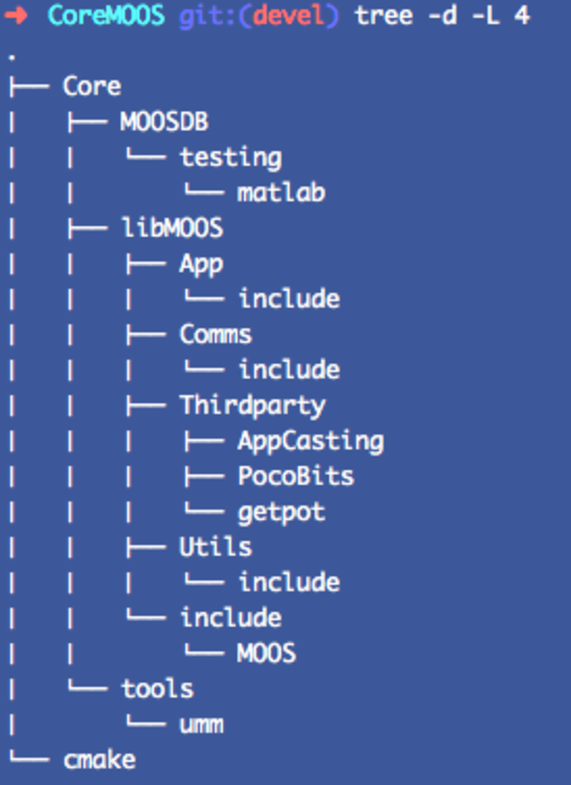
\includegraphics[width=0.5\columnwidth]{images/structure}\caption{Top-le\label{fig:Top-level-directory-structure}vel directory structure
for MOOS V10}
\end{figure}


You might be wondering where all the header files that used to be
in \texttt{MOOSGenLib} have gone. They are now in \texttt{``MOOS/libMOOS/Utils/{*}.h''.\vspace{5mm}}

\shadowbox{\begin{minipage}[t]{1\columnwidth}%
\textbf{Tip:} If you were previously including \texttt{``MOOSGenLibGlobalHelper.h''}
then you now need to include ``\texttt{MOOS/libMOOS/Utils/}MOOSUtilityFunctions\texttt{.h}''
instead (or use the compatibility mode described in Section \ref{sub:Building-V10}%
\end{minipage}}


\section{Developing with V10}


\subsection{Ethos}


\subsubsection{No code change required}

A lot of effort has been taken to make the users transition to MOOS
V10 painless. Indeed the goal was to make it possible to upgrade to
V10 without having to change any source code. The only thing a user
does need to do is link against the new library and this is made easy
with the revamped \texttt{CMake} build system. Of course good citizens
would probably be uncomfortable with living a legacy interface and
in time will want to upgrade. However the point is you can get started
with MOOS-V10 for zero overhead.


\subsubsection{Backward Compatibility (Mixed Systems)}

No assumption is made the all components of a MOOS system will be
upgraded. It is entirely possible to use a holy relic pre-V10 clients
or and old trusted MOOSDB with new or rebuilt software which has linked
against V10. The motivation here is to start using V10 you don't need
to rebuild everything. You could for example simply run the new MOOSDB
and you will still get improved performance. If you circumstances
dictate, you can even run the new \texttt{MOOSDB }in safe mode in
which it reverts to running the pre-V10 source code.


\subsection{Building V10 \label{sub:Building-V10}}


\subsubsection{The quickest way}

We shall begin where we should and check out a version of MOOS-V10
from a git repos. We will follow good practice and do an out of place
build - the source code will go in ``src'' and we will build in
``build''. We will also, after fetching the source switch to the
``devel'' branch because here we are living on the edge %
\footnote{if you want to know what branches are available type \texttt{git branch}%
}\texttt{.}

\begin{lstlisting}[style=Bash] 
pmn@mac:~$ mkdir core-moos-v10 
pmn@mac:~$ cd core-moos-v10
pmn@mac:~$ git clone git@github.com:themoos/core-moos.git src
pmn@mac:~$ cd src
pmn@mac:~$ git checkout devel 
pmn@mac:~$ cd ..
pmn@mac:~$ mkdir build
pmn@mac:~$ ccmake ../src
\end{lstlisting}

At this point you should, after hitting 'c' a couple of times be presented
with a CMake screen that looks like that shown in Figure \ref{fig:The-default-build}
(note some of the entries are platform dependent so don't worry if
what you see is not identical to this). If you simply want to link
your existing code against MOOS V10 without needing to worry about
the new header file structure then you will need to turn on \texttt{ENABLE\_V10\_COMPATIBILITY. }This
switch adds an additional set of include path to those exported by
the project, which have the same structure as those present in previous
(now legacy) versions of MOOS. If you ``include'' one of these files
they actually simply redirect to include header files residing in
the new structure. This is not a happy long term policy - you should
think if possible about updating your code - but there is much to
be said for not \emph{having }to change your code simply to use V10.
\vspace{5mm}

\shadowbox{\begin{minipage}[t]{1\columnwidth}%
\textbf{Tip: } Turn on \texttt{ENABLE\_V10\_COMPATIBILITY }to make
V10 appear to have the header structure of earlier versions. This
allows you to use V10 without needing to change any of your source
code%
\end{minipage}}

\begin{figure}
\begin{centering}
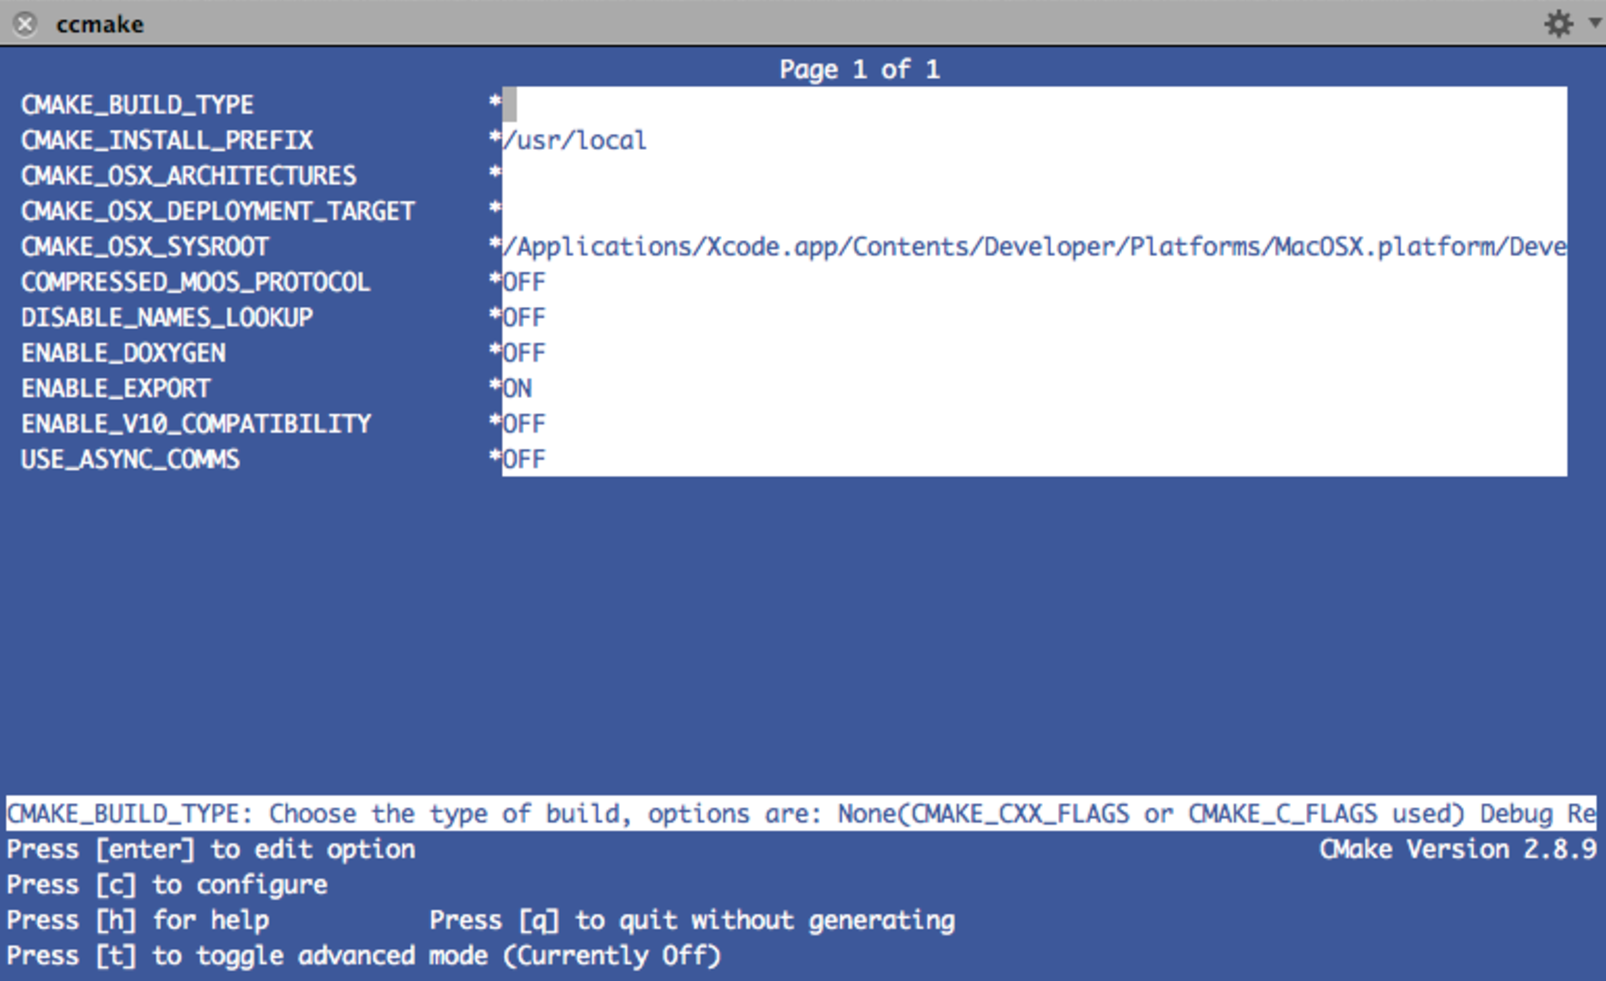
\includegraphics[width=0.9\columnwidth]{images/v10-simple-build}\caption{\label{fig:The-default-build}The default build screen for MOOS V10.
Note that by default USE\_ASYNC\_COMMS is off. If you want really
fast communications you should enable this.}

\par\end{centering}

\end{figure}


\vspace{5mm}

You are are now in a position to build the MOOS. So press 'c' until
'g' appears, then press 'g' and you are good to go. Then at the terminal
prompt type 'make' to build the project. Two directories should have
been created \textbf{bin} and \textbf{lib. }In lib you will see \texttt{libMOOS.a}
and in \texttt{bin} you will find the newly created \texttt{MOOSDB.}
If you run up the MOOSDB (by typing ./MOOSDB you should see output
similar to that in Figure \ref{fig:running-the-new-db}. You should
be able to use this \texttt{MOOSDB} to manage all communications with
any existing MOOS applications you have lying around - you should
not have to upgrade them. Again, at the risk of labouring a point,
MOOS-V10 is backwardly compatible in many senses. You are probably
wondering if just running this new DB by itself buys you anything.
The answer is yes, it does. Each client now has its own thread so
if you have dodgey comms between one client and the \texttt{MOOSDB
}this\texttt{ }ne'er-do-well client will not interfere with other
client DB interactions - it won't be able to hold them up\textbackslash{}%
\footnote{this was a big annoyance in earlier versions. There were occasions
in which a dodgey wireless connection between a client and a DB causes
all other clients connections to suffer. Misery%
}.\vspace{5mm}

\textbf{}%
\shadowbox{\begin{minipage}[t]{1\columnwidth}%
\textbf{Tip: }you can use the V10 \texttt{MOOSDB} with old MOOS applications
- you don't \textit{have} to recompile them. V10 is backwards compatible.%
\end{minipage}}

\vspace{5mm}

\begin{figure}
\begin{centering}
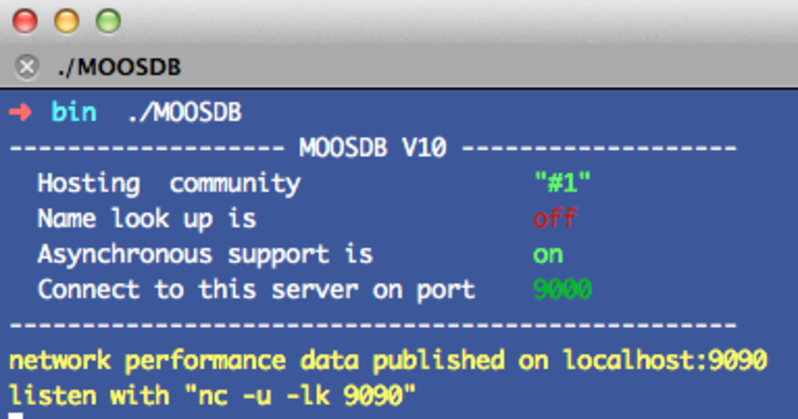
\includegraphics[width=0.5\columnwidth]{images/MOOSDBRunning}\caption{\label{fig:running-the-new-db}running the new MOOSDB}

\par\end{centering}

\end{figure}



\subsubsection{Changing \texttt{\#include} directives:}

If you are prepared to invest 30 minutes in committing to the new
MOOS V10 project structure then this section tells you what to do.
If you are as yet unsure if you want to upgrade, then don't bother
simply use the \texttt{ENABLE\_V10\_COMPATIBILITY }option in CMake
- this allows you to simply revert to old versions of MOOS without
lifting a finger.

The actions needed to upgrade are pretty simple. Where previously
you had something like \texttt{\#include ``MOOSLIB/MOOSCommClient.h''}
you now use \texttt{\#include ``MOOS/libMOOS/Comms/MOOSCommClient.h''. }The
following table will help you figure out how to include an particular
header.

\begin{center}
\begin{tabular}{|>{\raggedright}p{0.5\columnwidth}|>{\raggedright}p{0.5\columnwidth}|}
\hline 
Header & include prefix\tabularnewline
\hline 
\hline 
\texttt{\footnotesize MOOSAsyncCommClient.h MOOSMsg.h XPCEndian.h
XPCTcpSocket.h MOOSCommClient.h MOOSSkewFilter.h XPCException.h XPCUdpSocket.h
MOOSCommObject.h MOOSVariable.h XPCGetHostInfo.h MOOSCommPkt.h ServerAudit.h
XPCGetProtocol.h MOOSCommServer.h ThreadedCommServer.h XPCSocket.h} & \texttt{\#include ``MOOS/libMOOS/Comms/-{}-{}-.h''}\tabularnewline
\hline 
\texttt{\footnotesize ConsoleColours.h MOOSMemoryMapped.h MOOSTimeJournal.h
IPV4Address.h MOOSNTSerialPort.h MOOSUtilityFunctions.h InterpBuffer.h
MOOSPlaybackStatus.h MOOSUtils.h KeyboardCapture.h MOOSSafeList.h
NTSerial.h MOOSAssert.h MOOSSafeList.h\textasciitilde{} ProcessConfigReader.h
MOOSException.h MOOSScopedLock.h SafeList.h MOOSFileReader.h MOOSSerialPort.h
TMaxPair.h MOOSLinuxSerialPort.h MOOSThread.h TMinPair.h MOOSLock.h
MOOSThreadedTimeJournal.h ThreadPrint.h} & \texttt{\#include ``MOOS/libMOOS/Utils/-{}-{}-.h''}\tabularnewline
\hline 
\texttt{\footnotesize MOOSApp.h MOOSInstrument.h} & \texttt{\#include ``MOOS/libMOOS/App/-{}-{}-.h''}\tabularnewline
\hline 
\texttt{\footnotesize MOOSLib.h} & \texttt{\#include ``MOOS/libMOOS/MOOSLib.h''}\tabularnewline
\hline 
\end{tabular}
\par\end{center}


\subsection{Importing and Building Against MOOS-V10}

So now you have built the new MOOS. Next questions is ``how do you
link against it''. If you use \texttt{CMake} then this is trivial
you just need to insert the line \texttt{find\_package(MOOS 10)} in
your \texttt{CMakeList.txt} script. This goes and finds the latest
build you made of MOOS V10 (and only V10) and collects the correct
include paths, library names and library paths and puts them in the
following \texttt{CMake} variables:
\begin{description}
\item [{\texttt{MOOS\_INCLUDE\_DIRS}}] This contains the list of include
directories you need to include to find \texttt{MOOS V10} header files.
\item [{\texttt{MOOS\_DEPEND\_INCLUDE\_DIRS}}] This contains the list of
include directories which MOOS needs to find teh headers it depends
on (should be empty)
\item [{\texttt{MOOS\_LIBRARIES}}] This contains the precise library name
( absolute path) for \texttt{libMOOS }
\item [{\texttt{MOOS\_DEPEND\_LIBRARIES}}] This contains the absolute paths
for the libraries MOOS depends on (should be empty)
\end{description}
These variables can be used to import all you need to know about MOOS
into an external project. You can see how to do this in some the example
\texttt{CMakeLists.txt} file given below. Here we make an executable
called \texttt{example\_moos }, explicitly search for MOOS-V10, set
up include paths, set up an executable and finally indicate how to
link.

\doublebox{\begin{minipage}[t]{1\columnwidth}%
\begin{lstlisting}[basicstyle={\small},language=bash]
#this builds some code using MOOS
set(EXECNAME example_moos)

#find MOOS version 10 be explicit about version 10 so we don't
#find another old version
find_package(MOOS 10)

#what source files are needed to make this exectutable? 
set(SRCS  example_moos.cpp)

#where should one look to find headers?
include_directories( ${MOOS_INCLUDE_DIRS} ${MOOS_DEPEND_INCLUDE_DIRS})

#state we wish to make a computer program
add_executable(${EXECNAME} ${SRCS} )

#and state what libraries said program needs to link against
target_link_libraries(${EXECNAME} ${MOOS_LIBRARIES} ${MOOS_DEPEND_LIBRARIES})
\end{lstlisting}
%
\end{minipage}}


\subsubsection{How is MOOS found?}

You have probably noticed that you do not need to install MOOS V10
for \texttt{find\_package(MOOS V10)} to work. CMake simply appears
to automagically find the latest build directory. It is worth understanding
how this is done. CMake provides support for \texttt{find\_package
}by writing at build time to a file in \textasciitilde{}/.cmake/modules.
In this case because we are talking about \texttt{MOOS} there is a
file in \textasciitilde{}/.cmake/modules/MOOS (who's name is a whole
load of crazy letters) inside of which is the location to a file called
\texttt{MOOSConfig.cmake. }This file  is created in the build directory
when MOOS is configured. The find\_package directive imports \texttt{MOOSConfig.cmake}
(and from there \texttt{UseMOOS.cmake}) and this tells the importing
CMake instance how to use MOOS. 


\subsubsection{Trouble Shooting}

All the above should go smoothly but there have been instances reported
in which things go wrong - this is always due to previous installations
of MOOS and old configuration files hanging around. Executing the
following steps should help if you get into trouble
\begin{itemize}
\item clean down the \texttt{MOOS-V10} project (why not remove the whole
build directory?)
\item remove all contents of \texttt{\textasciitilde{}/.cmake/modules/MOOS}
\item remove any old copies of MOOSConfig.cmake you may have hanging around
in you build tree. Note that once upon a time, long ago there was
a \texttt{MOOSConfig.cmake} file checked into the source tree of MOOS-IvP.
This can cause all kinds of trouble......
\item If header files are not being found by you project:

\begin{itemize}
\item if your code previously worked with older versions of MOOS did you
change your source code to reflect the new locations of headers? Or,
if you really don't want to change you code, did you enable \texttt{V10\_COMPATIBILITY}
when you built MOOS-V10?
\end{itemize}
\end{itemize}

\section{Leveraging V10}

This section will explain how programmers and users of MOOS can leverage
some of the important and hopefully helpful new functionality in MOOS
V10.


\subsection{Asynchronous Comms}

This section explains new functionality offered in the V10 communications
classes which allow for very low latency communications between components.
This new facility allows one clients write of data to instigate a
read on all other clients who have previously expressed interest in
that data. This then is a departure from the model of a client having
to call in to the DB, deliver its post and while ``on the line'',
pick up and mail the DB has waiting for it. Of course we must stress
that the user has to opt in for this new functionality - there is
no imperative to run new code. To enable Asynchronous Comms in clients
derived from \texttt{CMOOSApp} you need to enable \texttt{USE\_ASYNC\_COMMS}
in a configure time in CMake.\vspace{5mm}. This flag makes the m\_\texttt{Comms}
member of \texttt{CMOOSApp} an \texttt{MOOS::MOOSAsyncCommsClient}
rather than a \texttt{CMOOSCommClient. }Note that you can have this
flag turned off and still use a\texttt{ MOOS::MOOSAsyncCommsClient}
object and the \texttt{MOOSDB} will service that object's interactions
appropriately.

\textbf{}%
\shadowbox{\begin{minipage}[t]{1\columnwidth}%
\textbf{Tip: }To enable fast asynchronous comms in MOOSApps you have
to turn \texttt{USE\_ASYNC\_COMMS} to \texttt{ON }when configuring
MOOS using CMake. %
\end{minipage}}


\subsubsection{Low Latency Communications via \texttt{MOOSAsyncCommClient}}

The key class is \texttt{MOOS::MOOSAsyncCommClient }which is a derivate
of the tried and test \texttt{CMOOSCommClient. }Its interface is identical\texttt{
}to\texttt{ CMOOSCommClient }and so the user should notice no progammatical
difference in using this client.%
\footnote{Indeed many users have little direct interaction with the communications
object preferring instead to operate withing the comfort of classes
derived from CMOOSApp which wraps the low level communications API. %
}

When a \texttt{MOOS::MOOSAsyncCommClient} connects to a V10 \texttt{MOOSDB}
it instigates some quite different behaviour. Firstly the DB spawns
two additional threads -one to handle reading from the client and
one to handle writing to the client. These threads are not \foreignlanguage{british}{synchronised}
- they operate independently pulling and pushing data from work queues
from within the DB itself. The client itself also has distinct read
and write threads - when a user posts some data it is added to a work
queue on which the read thread is waiting. The read thread pushes
this data to the DB and simply waits for another chunk of work to
appear on the queue. Similarly the clients read thread sits in a blocking
read on the socket linking it to the DB. When data arrives it is placed
into the clients ``mailbox'' and optionally a user callback is invoked.
Importantly, this architecture of each client having a read and write
thread at the client and \texttt{MOOSDB} ends, allows for data to
be pushed to clients at any time. Take for example the case of 50
clients all having subscribed for variable \texttt{``X''.} When
the 51st client publishes ``\textbf{X}'' this data can be instantly
placed on the outgoing queue of all 50 interested clients within th3
\texttt{MOOSDB}. Because the read threads on the clients are in a
blocking read they two an respond immediately leading to some very
responsive behaviour. Note also that if one of those clients has a
dodgey communications link to the DB this has not effect on the other
49 clients. This then is in stark contrast to the pre V10 releases
of MOOS. In section \ref{sec:Bench-Marks}some performance metrics
are given which highlight the difference in behaviour between V10
and previous incantations of the MOOS communications API.


\subsubsection{Supporting Iterate Modes in \texttt{MOOSApp}}

If MOOS is compiled with \texttt{USE\_ASYNC\_COMMS }then the \texttt{m\_Comms}
member of \texttt{CMOOSApp} becomes a MOOSAsyncCommClient and so all
communications will be using this new faster functionality. CMOOSApp
is designed to provide an easy to use framework in which to write
applications which leverage the MOOS communications API. The ability
for MOOSAsyncCommClients to have data pushed to them and invoke an
asynchronous callback affords the opportunity to augment the behaviour
of CMOOSApp to provide application developed with greater flexibility
and develop apps which respond quickly to communication events.

MOOS V10 offers three new configuration modes which are described
in the table below. The mode in which the application operates can
be set either in the applications configuration block (e.g by having
a line like \texttt{IterateMode = 2} or programmatically by calling
\texttt{SetIterateMode(REGULAR\_ITERATE\_AND\_COMMS\_DRIVEN\_MAIL)}
). These modes are supported by an additional configuration parameter
called MaxAppTick who's function is described in the table. This new
parameter can be set in the configuration file \texttt{MaxAppTick=100}
or passed as second parameter in \texttt{CMOOSApp::SetAppFreq(AppTick,MaxAppTick).\vspace{5mm}}

\begin{tabular}{|l|>{\raggedright}p{0.7\columnwidth}|}
\hline 
 & REGULAR\_ITERATE\_AND\_MAIL\tabularnewline
\hline 
\hline 
Summary & This mode is the default just as in pre-V10 releases Iterate() and
OnNewMail() are called regularly and if mail is available, in lock
step.\tabularnewline
\hline 
Configuration Block  & \texttt{IterateMode=0}\tabularnewline
\hline 
OnNewMail & called at most every \texttt{1/AppTick} seconds. If mail has arrived
\texttt{OnNewMail}() will be called just before \texttt{Iterate}()\tabularnewline
\hline 
Iterate & called every \texttt{1/AppTick} seconds. So if AppTick=10 \texttt{Iterate}()
will be called at 10Hz. \tabularnewline
\hline 
Role of AppTick & sets the speed of \texttt{Iterate()} in calls per second\tabularnewline
\hline 
Role of MaxAppTick & not used\tabularnewline
\hline 
Role of CommsTick & not used as communications are asynchronous\tabularnewline
\hline 
\end{tabular}

\vspace{5mm}

\begin{tabular}{|l|>{\raggedright}p{0.7\columnwidth}|}
\hline 
 & COMMS\_DRIVEN\_ITERATE\_AND\_MAIL\tabularnewline
\hline 
\hline 
Summary & The rate at which \texttt{Iterate} is called is coupled to the reception
of mail. As soon as mail becomes available \texttt{OnNewMail} is called
and is then followed by \texttt{Iterate}(). If no mail arrives for
\texttt{1/AppTick} seconds then iterate is called by itself. When
mail is arriving \texttt{Iterate()} and \texttt{OnNewMail()} are synchronous
- if \texttt{OnNewMail()} is called it will always be followed by
a called to \texttt{Iterate}()\tabularnewline
\hline 
Configuration Block  & \texttt{IterateMode=1}\tabularnewline
\hline 
OnNewMail & Called at up to \texttt{MaxAppTick} times per second. So if \texttt{MaxAppTick=100}
\texttt{OnNewMail()} will be called in response to the reception of
new mail at up to 100Hz.\tabularnewline
\hline 
Iterate & called at least \texttt{AppTick} times per second (if no mail) and
up to \texttt{MaxAppTick }times per second\tabularnewline
\hline 
Role of AppTick & sets a lower bound on the frequency at which \texttt{Iterate}() is
called. So if AppTick = 10 then \texttt{Iterate} will be called at
at least 10Hz\tabularnewline
\hline 
Role of MaxAppTick & sets an upper limit on the rate at which Iterate (and OnNewMail) can
me called. If \texttt{MaxAppTick}=0 both the speed is unlimited.\tabularnewline
\hline 
Role of CommsTick & not used as communications are asynchronous\tabularnewline
\hline 
\end{tabular}

\vspace{5mm}

\begin{tabular}{|l|>{\raggedright}p{0.7\columnwidth}|}
\hline 
 & REGULAR\_ITERATE\_AND\_COMMS\_DRIVEN\_MAIL\tabularnewline
\hline 
\hline 
Summary & Iterate is called regularly and \texttt{OnNewMail} is called when
new mail arrives. Iterate will not always be called after \texttt{OnNewMail}
unless it is scheduled to do so. In this way \texttt{OnNewMail} and
\texttt{Iterate} are decoupled.\tabularnewline
\hline 
Configuration Block  & IterateMode=2\tabularnewline
\hline 
OnNewMail & Called as soon as mail is delivered at up to \texttt{MaxAppTick }times
per second.\tabularnewline
\hline 
Iterate & called every AppTick times per second\tabularnewline
\hline 
Role of AppTick & sets the speed of \texttt{Iterate()} in calls per second as in REGULAR\_ITERATE\_AND\_MAIL\tabularnewline
\hline 
Role of MaxAppTick & limits the rate at which OnNewMail is called. If \texttt{MaxAppTick}=0
both the speed is unlimited. With a slight abuse of notation in this
mode \texttt{MaxAppTick }does not control \texttt{Iterate()} speed
at all - it simply limits the rate at which new mail can be responded
to\tabularnewline
\hline 
Role of CommsTick & not used as communications are asynchronous\tabularnewline
\hline 
\end{tabular}


\subsection{Wildcard Subscriptions}

MOOS-V10 extends the way in which clients can subscribe for data by
allowing ``wildcard subscriptions''. A client can register its interest
in variable whose name and source matches a simple regex pattern.
Currently only patterns containing {*} and ? wildcards are supported
with their usual meanings so ? means any single character and {*}
means any number of characters. An example will make this whole thing
clear and we will be using the new \texttt{CMOOSApp::Register( sVarPattern,
sAppPattern,dfInterval) }interface.

\begin{center}
\doublebox{\begin{minipage}[t]{1\columnwidth}%
\begin{lstlisting}[language={C++},showstringspaces=false]
bool MyApp::OnConnectToServer()
{
	//register for all variables ending with "image"
	//from any process with an name beginning with "camera_"
	Register("*image","camera_*, 0.0);

	//register for every single variable coming from a process
	//called "system_control"
	Register("*","sytem_control",0.0);

	//register for any variable beginning with "error_" and 
	//produced by a process with a nine letter name beginning
	//with "process_0" but please, only tell us at most twice
	//a second
	Register("error_*","process_0?", 2.0);
	return true;
}
\end{lstlisting}
%
\end{minipage}}
\par\end{center}

The logic which supports this new functionality is implemented at
the MOOSB and turns our to be a pretty useful and compact way to define
some fine granularity on what MOOSApp (or indeed CommsClient because
that is the fundamental communications object) receives. Of course
it can also be used to achieve blunderbuss subscriptions by subscribing
to all variables from a given process - \texttt{Register(``{*}'',ProcessName)
}- or even all variables from all processes - \texttt{Register(``{*}'',''{*}'')}
the ultimate wildcard. 


\subsection{Common Command Line Interface\label{sub:Common-Command-Line} }

\texttt{MOOSApp }now supports a whole set of command line options
which, by making a very small change to your code will make all your
programs which use MOOSApp respond in the same way %
\footnote{sadly this does require a code change as there is no other way to
get command line parameters in \texttt{CMOOSApp..}%
}. The upgrade is effected by invoking a new version of \texttt{CMOOSApp::Run}
which takes argc and argv as parameters:

\doublebox{\begin{minipage}[t]{1\columnwidth}%
\begin{lstlisting}[basicstyle={\small},language={C++}]
bool Run(const std::string &  sName,const std::string & sMissionFile, int argc, char * argv[]);
bool Run( const std::string &,int argc, char * argv[]); 
\end{lstlisting}
%
\end{minipage}}

This in turn populates a member variable within \texttt{CMOOSApp}
called \texttt{m\_CommandLineParser }which is used internally to parse
the following command line variables and flags.

\doublebox{\begin{minipage}[t]{1\columnwidth}%
\begin{lstlisting}[basicstyle={\small}]
variables:   
--moos_app_name=<string>    : name of application
--moos_name=<string>        : name with which to register with MOOSDB   
--moos_file=<string>        : name of configuration file   
--moos_host=<string>        : address of machine hosting MOOSDB   
--moos_port=<number>        : port on which DB is listening    
--moos_app_tick=<number>    : frequency of application (if relevant)    
--moos_max_app_tick=<number>: max frequency of application (if relevant)    
--moos_comms_tick=<number>  : frequency of comms (if relevant)    
--moos_iterate_Mode=<0,1,2> : set app iterate mode 
--moos_time_warp=<number>   : set moos time warp

flags:   
--moos_iterate_no_comms     : enable iterate without comms    
--moos_filter_command       : enable command message filtering    
--moos_no_sort_mail         : do not sort mail by time    
--moos_no_comms             : do not start communications    
--moos_quiet                : do not print banner information
--moos_quit_on_iterate_fail : quit if iterate fails 
help:   
--moos_print_example        : print an example configuration block    
--moos_print_interface      : describe the interface (subscriptions/pubs)   
--moos_print_version        : print the version of moos in play    
--moos_help                 : print help on moos switches   
--help                      : print help on moos messages and custom help
\end{lstlisting}
%
\end{minipage}}

\textbf{}%
\shadowbox{\begin{minipage}[t]{1\columnwidth}%
\textbf{Tip: }To enable common command line parsing call\\
\texttt{CMOOSApp::Run(moos\_name,mission\_file,argc,argv)} 

or a variant when you start a \texttt{MOOSApp}%
\end{minipage}}


\subsubsection{New Command Line Related Functions to Overload}

MOOS-V10 adds new virtual functions to \texttt{CMOOSApp} which can
be overloaded to process additional command line parameters if argc,
and argv have been passed to your \texttt{CMOOSApp} derived class.
\begin{itemize}
\item \texttt{OnProcessCommandLine() }is called so you can do additional
command line parsing
\item \texttt{OnPrintExampleAndExit()} is called when \texttt{-{}-moos\_print\_example}
is present on the command line. The intent is you use this function
to print out an example configuration file block.
\item \texttt{OnPrintInterfaceAndExit()} is called when \texttt{-{}-moos\_print\_interface}
is present on the command line. The intent is you use this function
to print out details of the processes subscriptions and publications.
\item \texttt{OnPrintHelpAndExit() }is called when \texttt{-{}-moos\_help}
or\texttt{ -{}-help} is present on the command line. The intent here
is that you print out help for additional command line parameters
inside this function.
\end{itemize}

\subsubsection{The Publication of CPU load}

In a \texttt{CMOOSApp}, every application publishes a status message.
You get to add detail to this message by overloading (and within your
overload calling) \texttt{CMOOSApp::MakeStatusString(). }The default
message now contains CPU load information for that process expressed
as a percentage of available cpu grunt. There is a standalone class
which can be used to acquire CPU information - it is \texttt{MOOS::ProcInfo.}


\subsection{MOOSDB Interface Improvements}


\subsubsection{Command Line}

Its pretty dull to only be able to configure processes from a script.
\texttt{MOOSDB} now supports a better command line interface which
allows you to set the port it is serving on and various other configurations.
All accessed via \texttt{./MOOSDB -{}-help}

\doublebox{\begin{minipage}[t]{1\columnwidth}%
\begin{lstlisting}
>>pmn@mac  ./MOOSDB --help
MOOSDB command line help:
--moos_file=<string>                  specify mission file name 
--moos_port=<positive_integer>        specify server port number  
--moos_timewarp= <positive_float>     specify time warp 
--moos_community=<string>             specify community name 
--moos_timeout=<positive_float>       specify client timeout 

--response=<string-list>			  specify client response times <name:response_ms,...>
-s (--single_threaded)                run as a single thread 
-d (--dns)                            run with dns lookup 
--webserver_port=<positive_integer>   run webserver on given port 
-h    (--help)                        print help and exit
\end{lstlisting}
%
\end{minipage}}


\subsubsection{Configuring Client Response Times}

The MOOSDB has some inbuilt security controls that are designed to
prevent a rogue, ill mannered client to hog resources. It seems improper
that a random client joining a community can decide to send 10 million
messages persecond and because of that, reduce the performance of
other clients. On the other hand it seems inappropriate to disallow
all clients for all time very rapid performance simply because of
a percieved risk. The solution offered in MOOS-V10 is that the MOOSDB
by default offers premiums service to all comers %
\footnote{if they are using the AsyncComms%
} - in other words every client will be serviced as soon as possible
and all clients will be have data pushed to them as soon as possible.
However the launcher of the \texttt{MOOSDB} may choose to restrict
response times for clients- this has the effect of having each transaction
with the DB contain more indvidual messages and prevents rogue clients
being disruptive. Even introducing a repsonse time of 10ms can have
a marked increase in performance for a very heavily loaded system.
It is also possible to control which clients should be throttled and
which should not.

\begin{lstlisting}[style=Bash] 
pmn@mac:~$ ./MOOSDB --response=*:20
pmn@mac:~$ ./MOOSDB --response=VisualOdometry:10
pmn@mac:~$ ./MOOSDB --response=Camera??:10,VisualOdometry:10,*:20
\end{lstlisting}

In the above, the first example sets all clients to have a minimum
reposnse time of 20ms. The second example expicitly sets a client
called \texttt{VisualOdometry }to have a 10ms response while all others
have the default of 0ms (instant response). The final example has
any client whos name begins with ``Camera'' followed by two characters
set to 10ms and \texttt{VisualOdometry} at 10ms and every other client
at 20ms.


\subsubsection{Specifying When Clients are Assumed Dead}

\texttt{MOOSDB} has alway been suspicious of clients that unexpectedly
go quiet (the comms thread, which operates behind the scenes, stops
working) and it will disconnect them. However its pretty annoying
if you are debugging an application and because you could not solve
you problem in 5 seconds, the DB disconnects your application and
so differnt behaviour is invoked while debugging (the app will try
to reconnect as soon the debugger sets teh application free). In V10,
\texttt{MOOSDB} has the \texttt{-{}-moos\_timeout} option which allows
you to specify the time in seconds the DB should tolerate a silent
client. Set this to a big number when you are debugging.


\subsubsection{Live Network Audit}

Sometimes its nice to quickly get a summary of the network performance
of the MOOSDB and the clients it supports. The MOOS V10 DB supports
a very lightweight way to see how things are going. When the DB starts
you'll see it print out something like \texttt{``network performance
data published on localhost:9090 listen with \textquotedbl{}nc -u
-lk 9090\textquotedbl{} ''. }So if you follow this advice and in
a terminal start \texttt{netcat (which is the ``nc'' command)} listening
on port 9090 it will receive UDP packets which contain performance
data. Here is an example output - don't be put off by the fact that
the client names are actually numbers in this case - that just happens
to be the naming scheme this community was running. The network summary
packet is sent once a second and contains valid statistics for that
last second.

\begin{center}
\doublebox{\begin{minipage}[t]{1\columnwidth}%
\begin{lstlisting}
  client name   pkts in  pkts out  msgs in  msgs out   B/s in  B/s out
         0        20        17      20	  20		  1207      1227
         1        19        19      19	  19		  1216      2177
     total        39        36      39      39		  2423	  3404
\end{lstlisting}
%
\end{minipage}}
\par\end{center}


\subsection{Backwards Compatibility }

MOOS V10 was designed to offer complete backwards compatibility between
all versions of MOOS. You should be able to run legacy code with modern
clients and old DB's alike. You should be able to run heterogenous
communities with any combination of pre V10 and V10 applications.
The table below shows the options available for different combinations.\vspace{5mm}

\begin{tabular}{|c|c|c|c|c|c|c|}
\hline 
Client & MOODB & OK & Async. Comms & Synch. Comms & Multithreading DB & Single Threaded DB\tabularnewline
\hline 
\hline 
Pre10 & Pre10 & \CheckmarkBold{} & \XSolidBrush{} & \CheckmarkBold{} & \XSolidBrush{} & \CheckmarkBold{}\tabularnewline
\hline 
Pre10 & V10 & \CheckmarkBold{} & \XSolidBrush{} & \CheckmarkBold{} & \CheckmarkBold{} & \CheckmarkBold{}\tabularnewline
\hline 
V10 & Pre V10 & \CheckmarkBold{} & \XSolidBrush{} & \CheckmarkBold{} & \XSolidBrush{} & \CheckmarkBold{}\tabularnewline
\hline 
V10 & V10 & \CheckmarkBold{} & \CheckmarkBold{} & \CheckmarkBold{} & \CheckmarkBold{} & \CheckmarkBold{}\tabularnewline
\hline 
\end{tabular}


\subsubsection{Retreating back to the known}

It is also possible to force the MOOSDB to behave (ie run almost exactly
the same code) as previous versions did. So if you are using the V10
code base but want to return to the good old days the recipe is:
\begin{enumerate}
\item Run MOOSDB with the single threaded switch .\texttt{/MOOSDB -s}
\item Make sure you compile V10 with USE\_ASYNC\_COMMS=OFF and ENABLE\_V10\_COMPATIBILITY=ON
\end{enumerate}

\section{Bench Marks and Testing Tools\label{sec:Bench-Marks}}


\subsection{Testing with \texttt{umm}}

Sometimes its attractive to be able to simply to fire up a program
from the command line that subscribes to an publishes messages of
your choosing - just to test the MOOS Communications facilities and
explore performance. There is a tool called \texttt{umm }%
\footnote{if you forget this name you may end up saying ``umm...'' as you
recall you are looking to ``\textbf{u} \textbf{m}onitor \textbf{m}oos''%
} which is designed to achieve just this and it also allows you to
simulate applications crashing or operating with high latency networks.
It is entirely configurable from the command line and has the following
options (in addition to the standard MOOS ones described in Section
\ref{sub:Common-Command-Line} which you use to set MOOS parameters
to something other than their default value).

\begin{lstlisting}
Publication and Subscription  settings:   
-s=<string>  : list of subscriptions as var_name@period 
-w=<string>  : list of wildcard subscriptions as var_pattern:app_patter@period   
-p=<string>  : list of publications as var_name[:optional_binary_size]@period 
--latency    : show latency (time between posting and receiving)   
--verbose    : verbose output
--bandwidth  : show bandwidth statistics

spying helpful settings:   
--spy          		: spy on all variables at 1Hz   
--spy_all          	: spy on all variables   
--spy_proc=<string>    : spy on all variables from a named processes

Network failure simulation:   
--simulate_network_failure=<numeric>   
			: enable simulation of network/app failure   
--network_failure_prob=<numeric>       
			: probability of each DB interaction having network failure [0.1]   
--network_failure_time=<numeric>       
			: duration of network failure [3s]   
--application_failure_prob=<numeric>   
			: probability of application failing during DB-communication [0]
\end{lstlisting}


Some examples are probably useful at this point. 


\subsubsection{Publishing Variables with \texttt{umm}}

So if we wanted to send the variable \texttt{X }at 20Hz we would type:

\begin{lstlisting}[style=Bash] 
./umm -p=X@20 
\end{lstlisting}

and in this case X would be a numeric (MOOS\_DOUBLE) variable. Imagine
now we wanted to try sending binary data. We would be compelled to
write:

\begin{lstlisting}[style=Bash] 
./umm -p=X@20,Y:10000@15 
\end{lstlisting}

and this would write Y as 10K of binary data a 15 Hz. 


\subsubsection{Subscribing with \texttt{umm}}

We can also subscribe to data

\begin{lstlisting}[style=Bash] 
./umm -p=X@20,Y:10000@15 -s=Z@8,X@0 --verbose
\end{lstlisting}

which subscribes for every issue of X (which we are publishing ourself!)
and also Z at to 8 Hz. Note that $0Hz$ is overloaded to mean subscribe
to everything. The verbose flag simply adds some printing so you can
check progress. 


\subsubsection{Wildcard subscriptions with umm}

You can of course also access the wildcard subscription service offered
by MOOS 10. This is done via the \texttt{-w} switch. For example

\begin{lstlisting}[style=Bash] 
./umm -p=X@20,Y:10000@15 -s=Z@8,X@0 --verbose -w='*:ProcA@0'
\end{lstlisting}

does all the above and subscribes to all messages from a process called
\texttt{\textbf{ProcA}}. Note the use of the single quotation to stop
the shell interpreting the wilcard '{*}'. Of course you can build
complicated filters this way

\begin{lstlisting}[style=Bash] 
./umm --verbose --bandwidth -w='*:ProcA@1,battery_*:monitor_?'
\end{lstlisting}

which subscribes to everything from ProcA at 1Hz and every issue of
any variable which begins with ``battery\_'' from any process which
whose name begins with ``monitor\_'' and ends with any single character.
This example also prints out these messages and also bandwidth statistics.
You can also use the network failure simulation switches to test MOOS's
ability to deal with errant clients.

\textbf{}%
\shadowbox{\begin{minipage}[t]{1\columnwidth}%
\textbf{Tip: }you can use \texttt{umm} to watch all MOOS traffic try
\texttt{./umm -w='{*}:{*}@0' -{}-verbose }to see everything or \texttt{./umm
-w='{*}:ProcA@1' }to see everything from \texttt{ProcA} at 1Hz.%
\end{minipage}}


\subsubsection{Generic Spying with umm}

Building on the above \texttt{umm }offers some short cuts for spying
on the publications of the community at large

\begin{lstlisting}[style=Bash] 
./umm --spy
./umm --spy_all
./umm --spy_proc=GPS,INS
\end{lstlisting}

here, in the first example, we have asked to be told about all publications
every second. The second example lists each and every publication
and the last listens only to publications from the specified processes.


\subsubsection{Logging with umm}

Sometime its nice to simply be able to capture messages around the
community from the command line. \texttt{umm} can help. By using the
\texttt{-{}-log=file\_name }switch all captured messages are written
to a a text file.

\vspace{5mm}


\subsection{Profiling with \texttt{async\_test}}

It is useful to have some statistical sense of performance. Its nice,
when you have built V10 to have some sense of latencies and throughputs.
In the directory build directory \texttt{bin }you will find an executable
called \texttt{async\_test }which can be used to do some benchmarking.
The program \texttt{async\_test} instantiates a configurable number
$2N$ of Comms Clients N of which are AsyncCommsClients and the other
N of which are pre-V10 clients. Client $C_{j}$ is asynchronous if
j is even. All clients register with the \texttt{MOOSDB} under the
numerical name \texttt{j (so ``1'',''2'' }etc\texttt{)} Client
$C_{0}$ is Asynchronous and is charged with regularly posting a variable
``\texttt{X}'' or configurable size to the MOOSDB. All clients including
$C_{0}$ subscribe to \texttt{X. }The time in milliseconds between$C_{0}$
sending and client $C_{j}$ receiving the data is logged to file \texttt{asynctest.log
}as a plain text matrix :

\[
\begin{array}{ccccc}
0 & \tau_{1}^{0} & \tau_{2}^{0} & \tau_{3}^{0} & \cdots\\
1 & \tau_{1}^{1} & \tau_{1}^{1} & \tau_{1}^{1} & \cdots\\
2 & \tau_{1}^{0} & \tau_{1}^{0} & \tau_{1}^{0} & \cdots\\
\vdots & \vdots & \vdots & \vdots & \ddots
\end{array}
\]


where $^{j}\tau_{i}$ is the $i^{th}$ latency for client $C_{j}$
and each row begins with $j$ . The test can be run for a configurable
number of seconds after which histograms of performance for each kind
of client can be produced. The options for \texttt{uDBAsyncTest} are
below.

\begin{lstlisting}

V10 performance and compatibility testing
  -p              : test period in seconds (20 seconds default)
  -m              : send test data every m milliseconds (default 100 ms)
  -c              : number of clients to instantiate (default 40)
  -s              : size of data to send default (default 1024 bytes)

Example Usage:  test for 15 seconds with 20 clients and sending 100K every 50 ms   
	
	./async_test  -p=15 -c=20 -m=50 -s=100000
\end{lstlisting}


The figures on the following pages give the probability distributions
over message latencies under different conditions (specified in caption).
For example Figure \ref{fig:Histograms-of-latencies-5C-20Hz} was
generated with 

\begin{lstlisting}
./async_test  -p=20 -c=5 -m=50 -s=1000
./async_test  -p=20 -c=5 -m=50 -s=10000
./async_test  -p=20 -c=5 -m=50 -s=10000
./async_test  -p=20 -c=5 -m=50 -s=1000000
\end{lstlisting}


Which fires 1K,10K 100K and 1MB messages at 20Hz (every 50ms) to the
DB which are immediately routed to 5 clients. This sort of testing
not only gives a sense of latencies but also a sense of the total
through-put of the system. For the results given here the \texttt{MOOSDB
}was on the same machine as .\texttt{/}async\_test\texttt{ }which
means we are testing logic speed not network speed. The results are
gathered on a 2.2GHz Intel Core i7 Mac book Pro running OS X 10.8
and all code was built in Debug (so these results are conservative).
Its pretty clear that V10 clients offer between one and two orders
of magnitude improvement in performance in terms of latency.

\begin{center}
\begin{figure}
\subfloat[Sending and receiving 1KB messages. ]{\begin{centering}
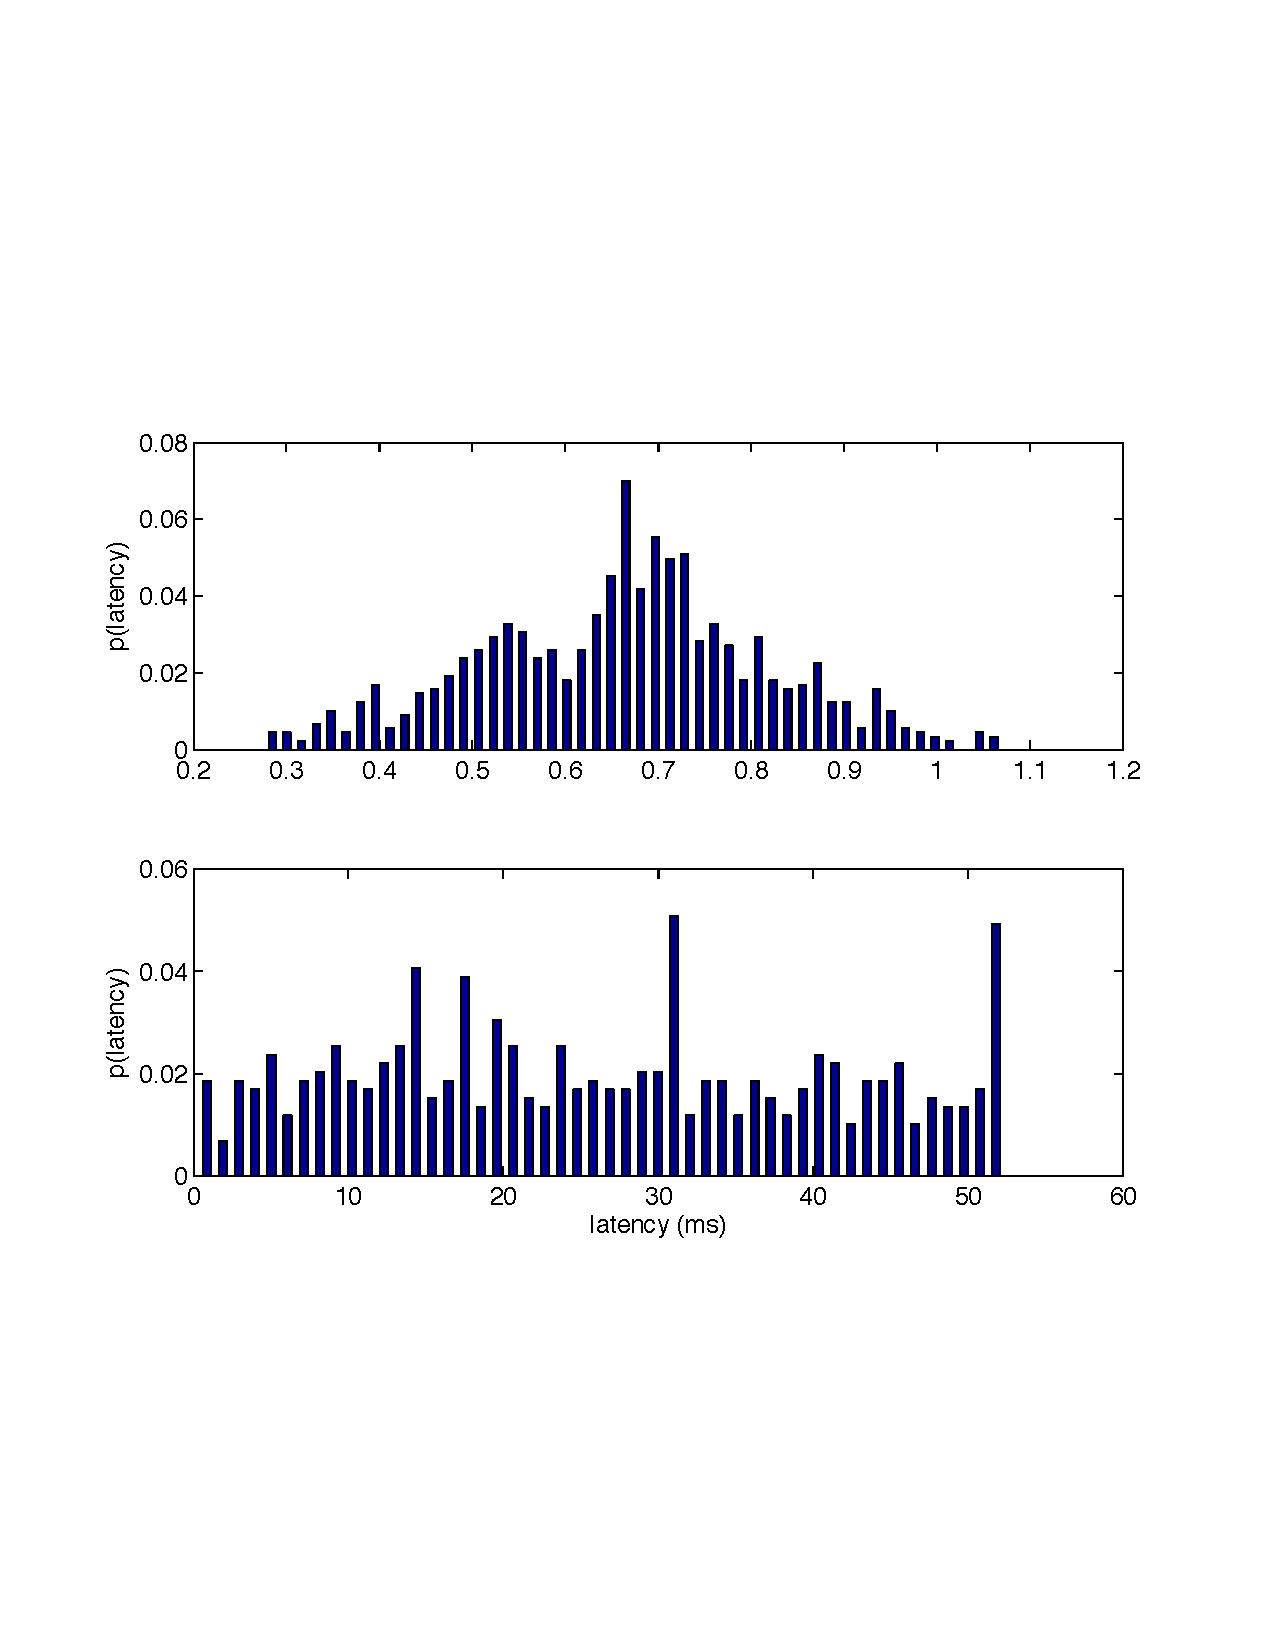
\includegraphics[width=0.45\columnwidth]{images/test_results/asynctest_5_clients_1k_20Hz}
\par\end{centering}

}\hfill{}\subfloat[Sending and receiving 10KB messages. ]{\centering{}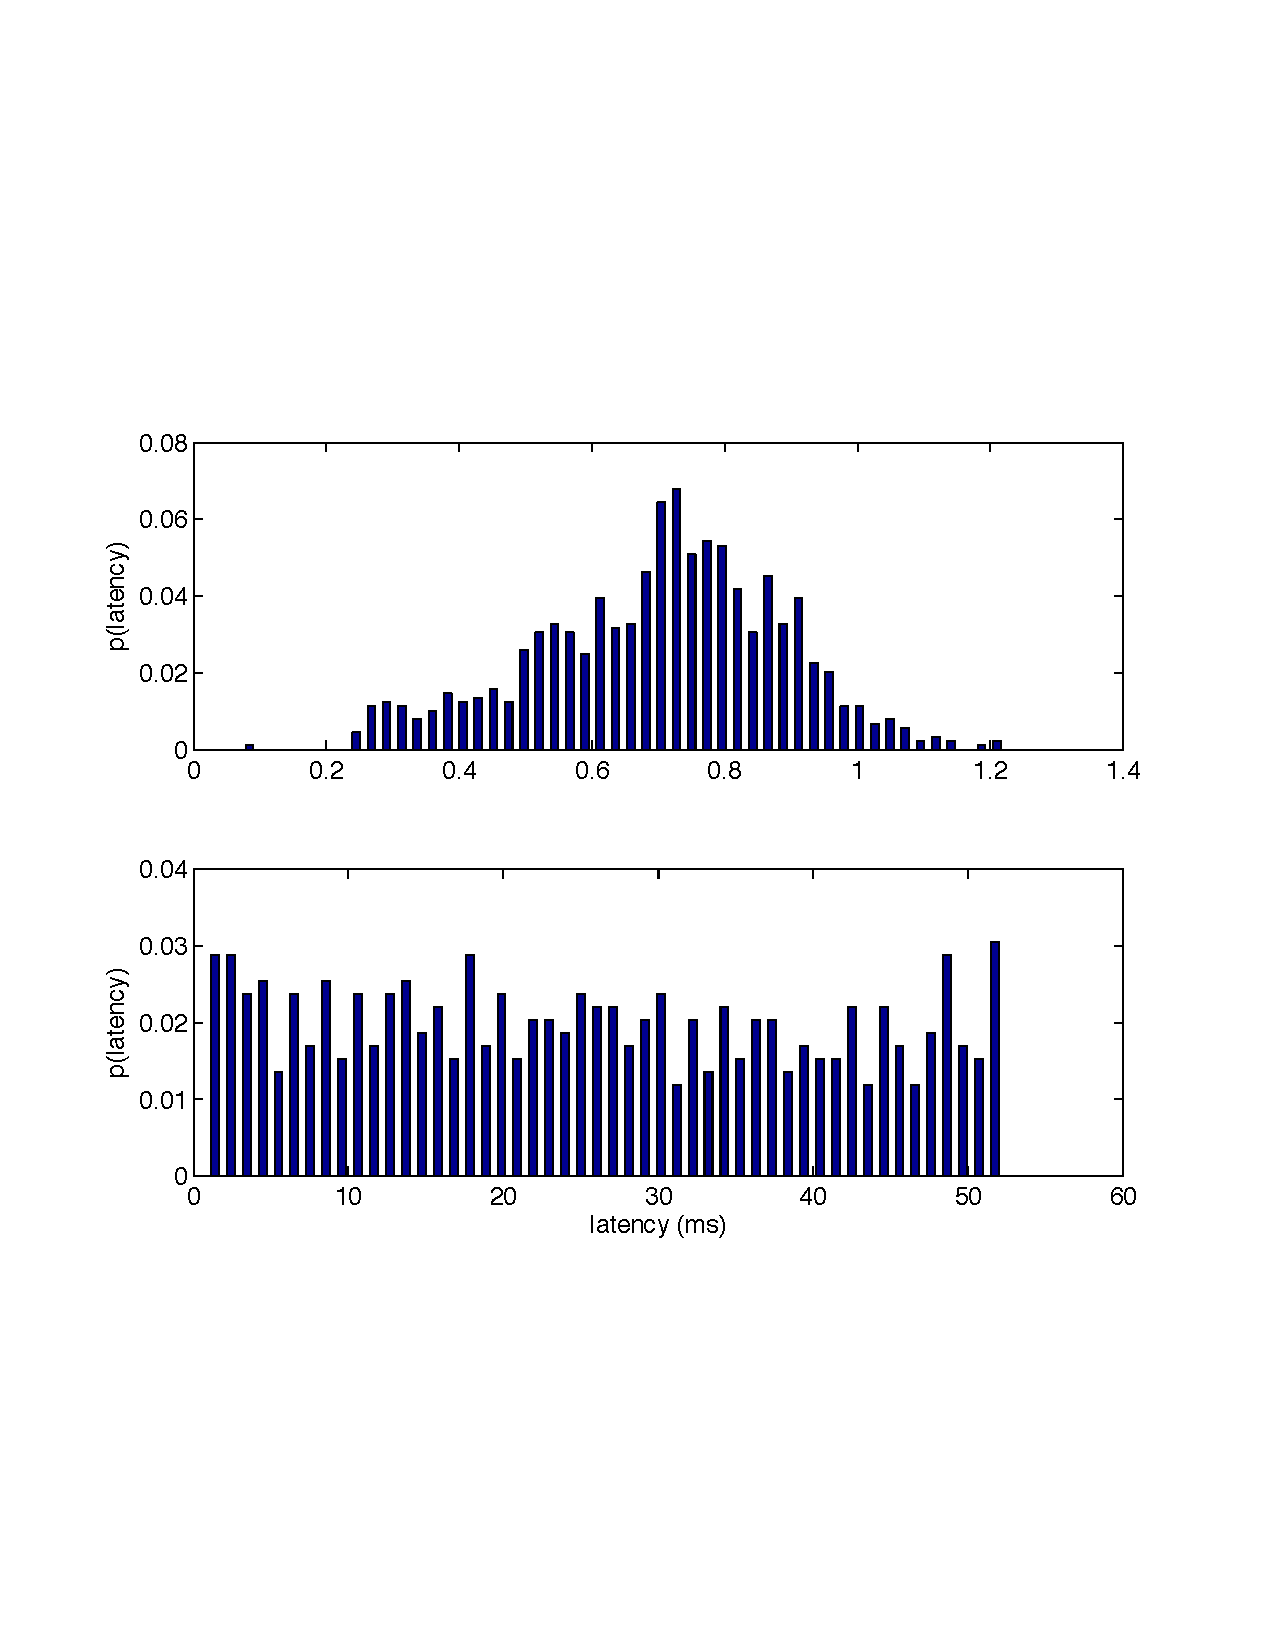
\includegraphics[width=0.45\columnwidth]{images/test_results/asynctest_5_clients_10k_20Hz}}\hfill{}\subfloat[Sending and receiving 100KB messages. ]{\begin{centering}
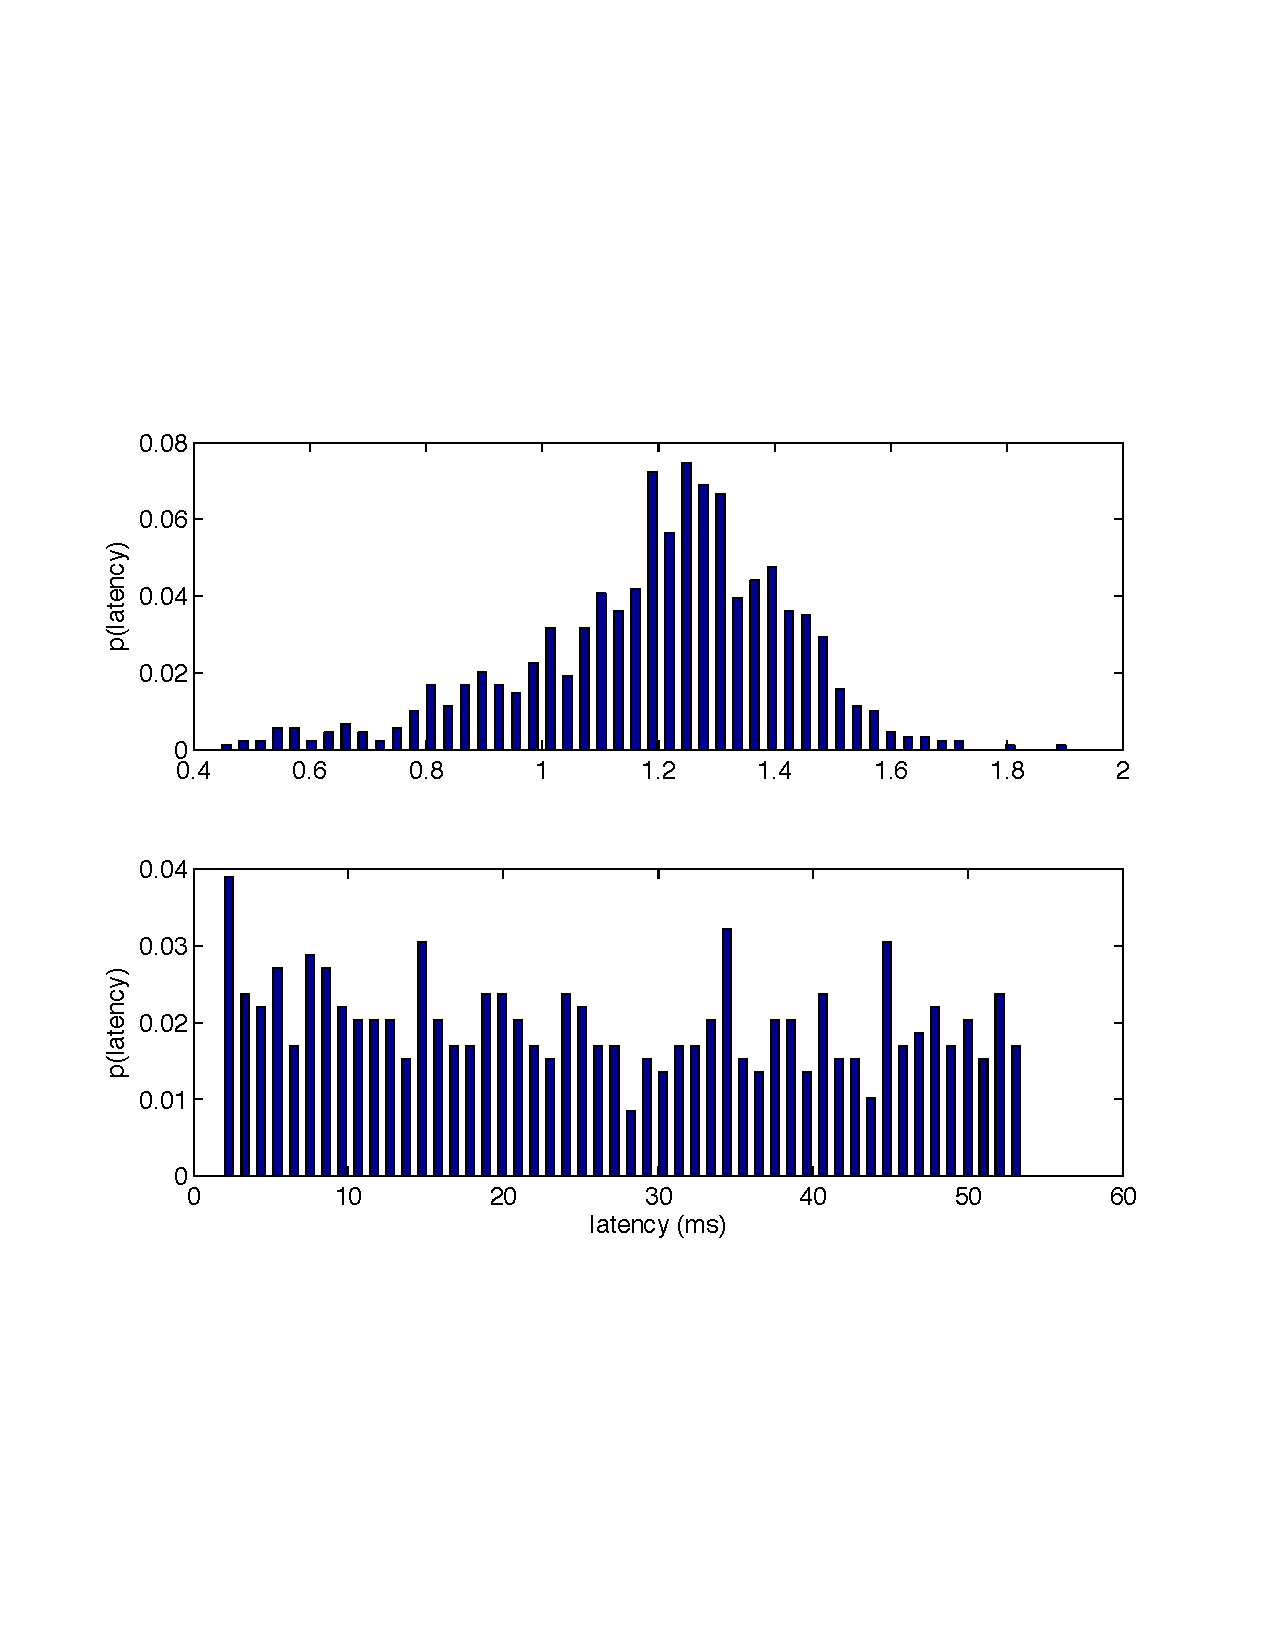
\includegraphics[width=0.45\columnwidth]{images/test_results/asynctest_5_clients_100k_20Hz}
\par\end{centering}

}\hfill{}\subfloat[Sending and receiving 1MB messages]{\centering{}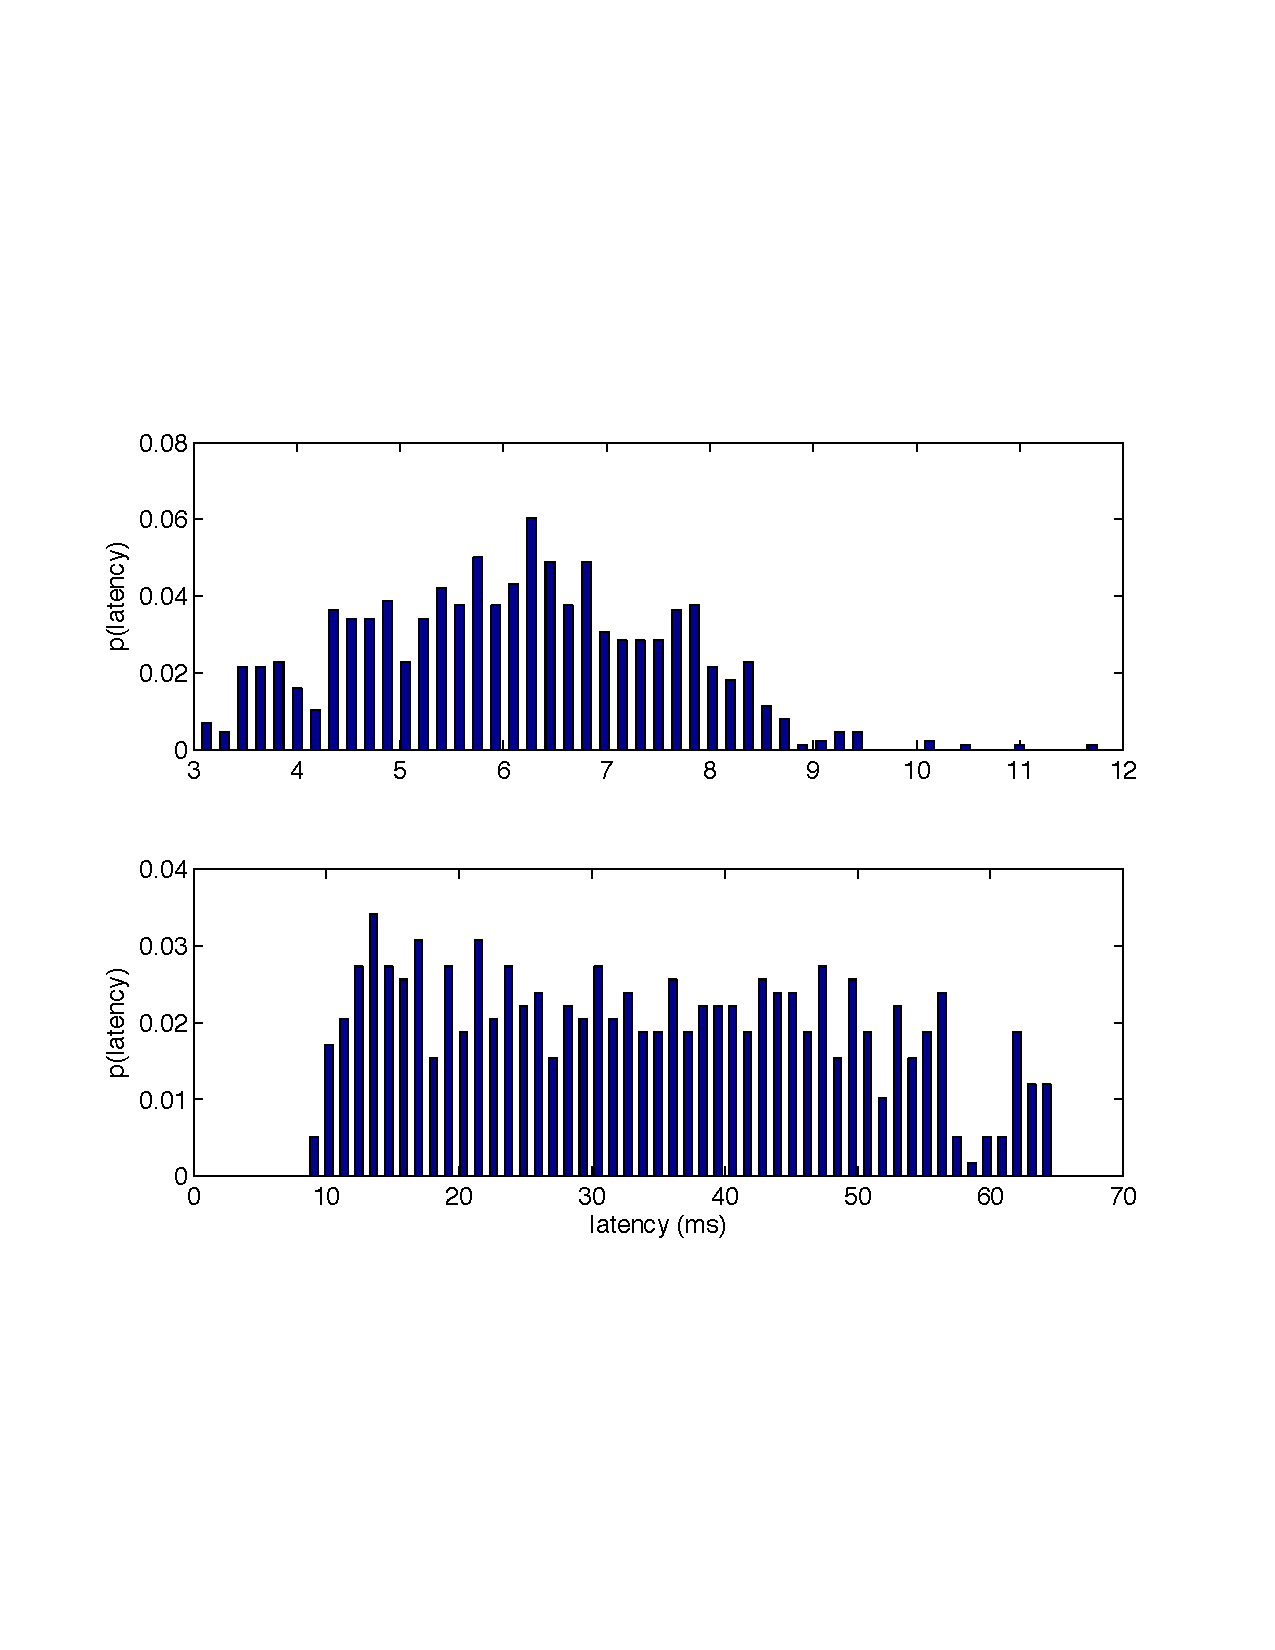
\includegraphics[width=0.45\columnwidth]{images/test_results/asynctest_5_clients_1M_20Hz}}\caption{Histograms of latencies between sending and receiving 1KB,10KB, 100KB
and 1MB messages. Messages are sent to 5 clients at 20Hz. Top figures
are for asynchronous clients lower figures are for pre V10 clients
with a comms-tick set 20Hz. All cases are using the \texttt{V10 MOOSDB.}
As an example of total throughput take the example of sending 100KB
messages to 5 clients 20 times a second so 100K{*}5{*}20=10MB/s.\label{fig:Histograms-of-latencies-5C-20Hz}}
\end{figure}

\par\end{center}

\begin{center}
\begin{figure}
\subfloat[Sending and receiving 1KB messages. ]{\centering{}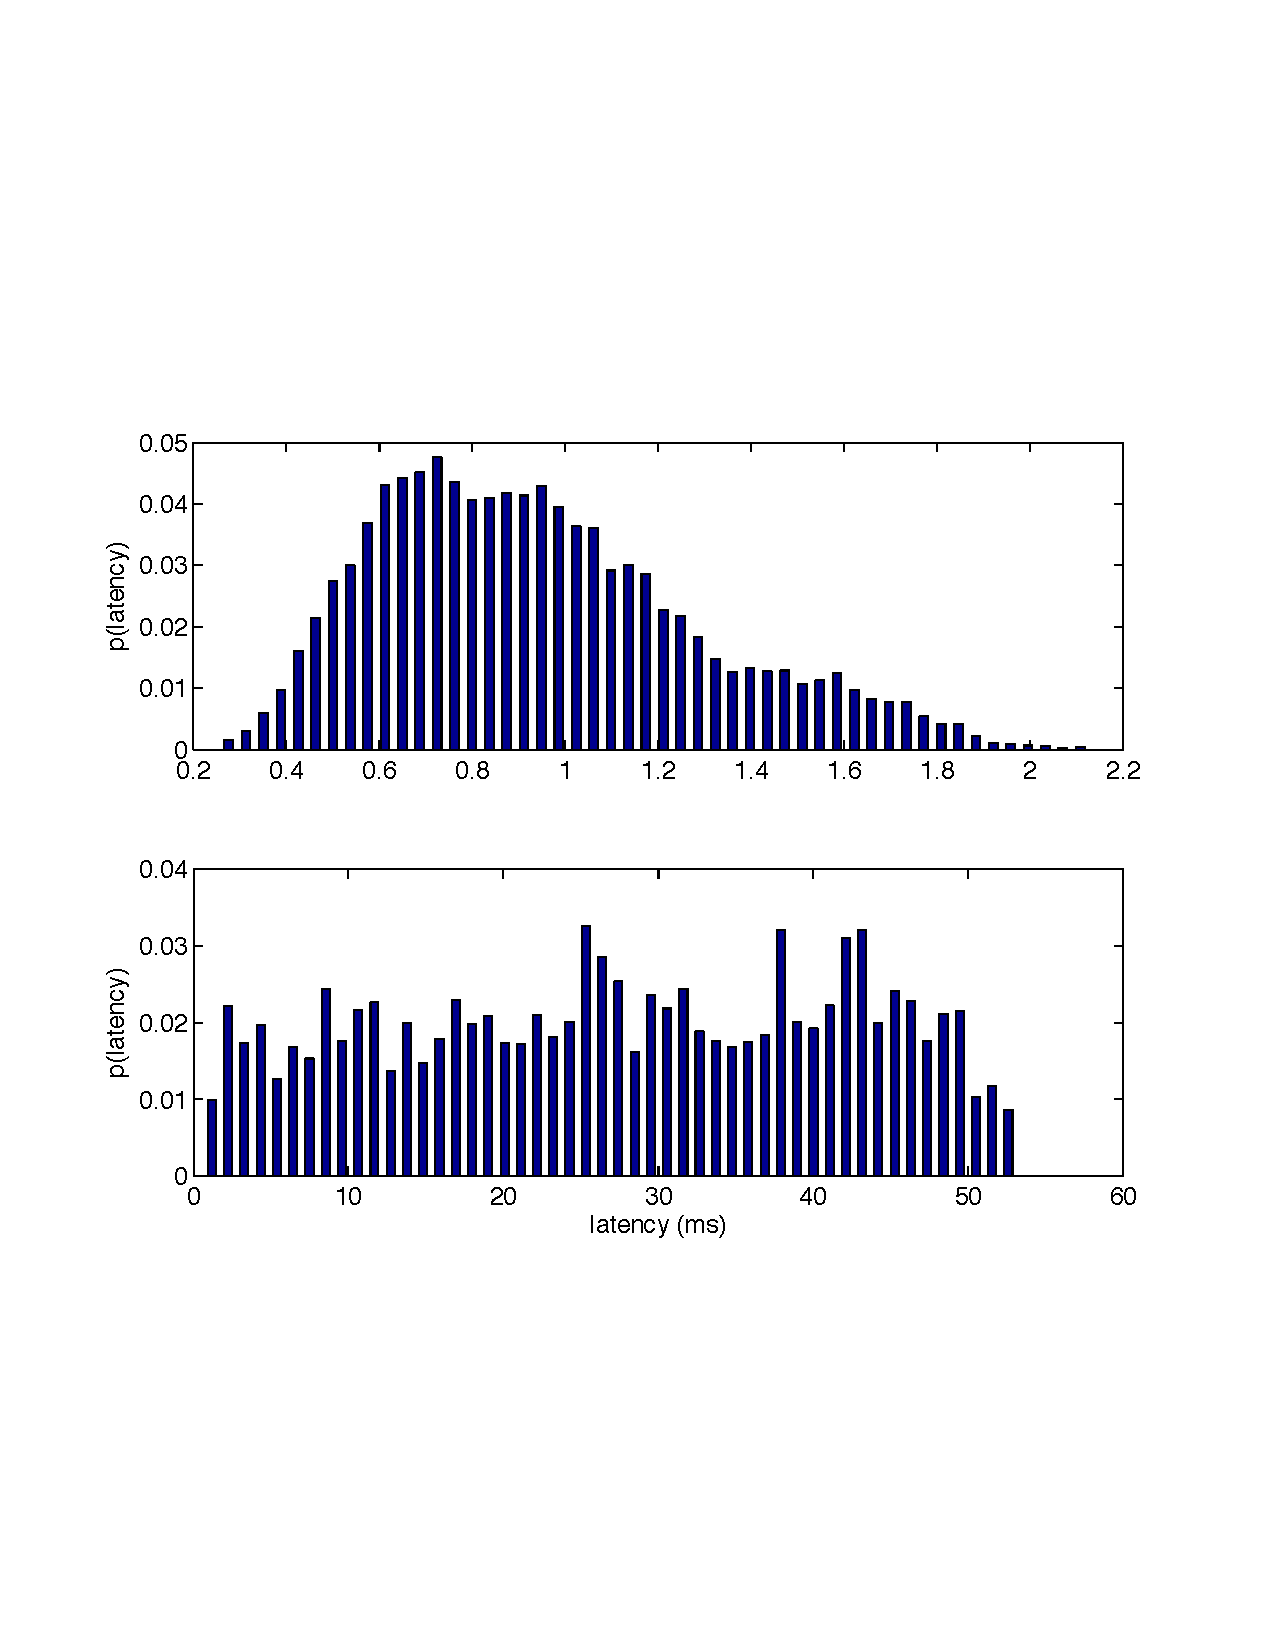
\includegraphics[width=0.45\columnwidth]{images/test_results/asynctest_50_clients_1k_20Hz}}\hfill{}\subfloat[Sending and receiving 10KB messages. ]{\centering{}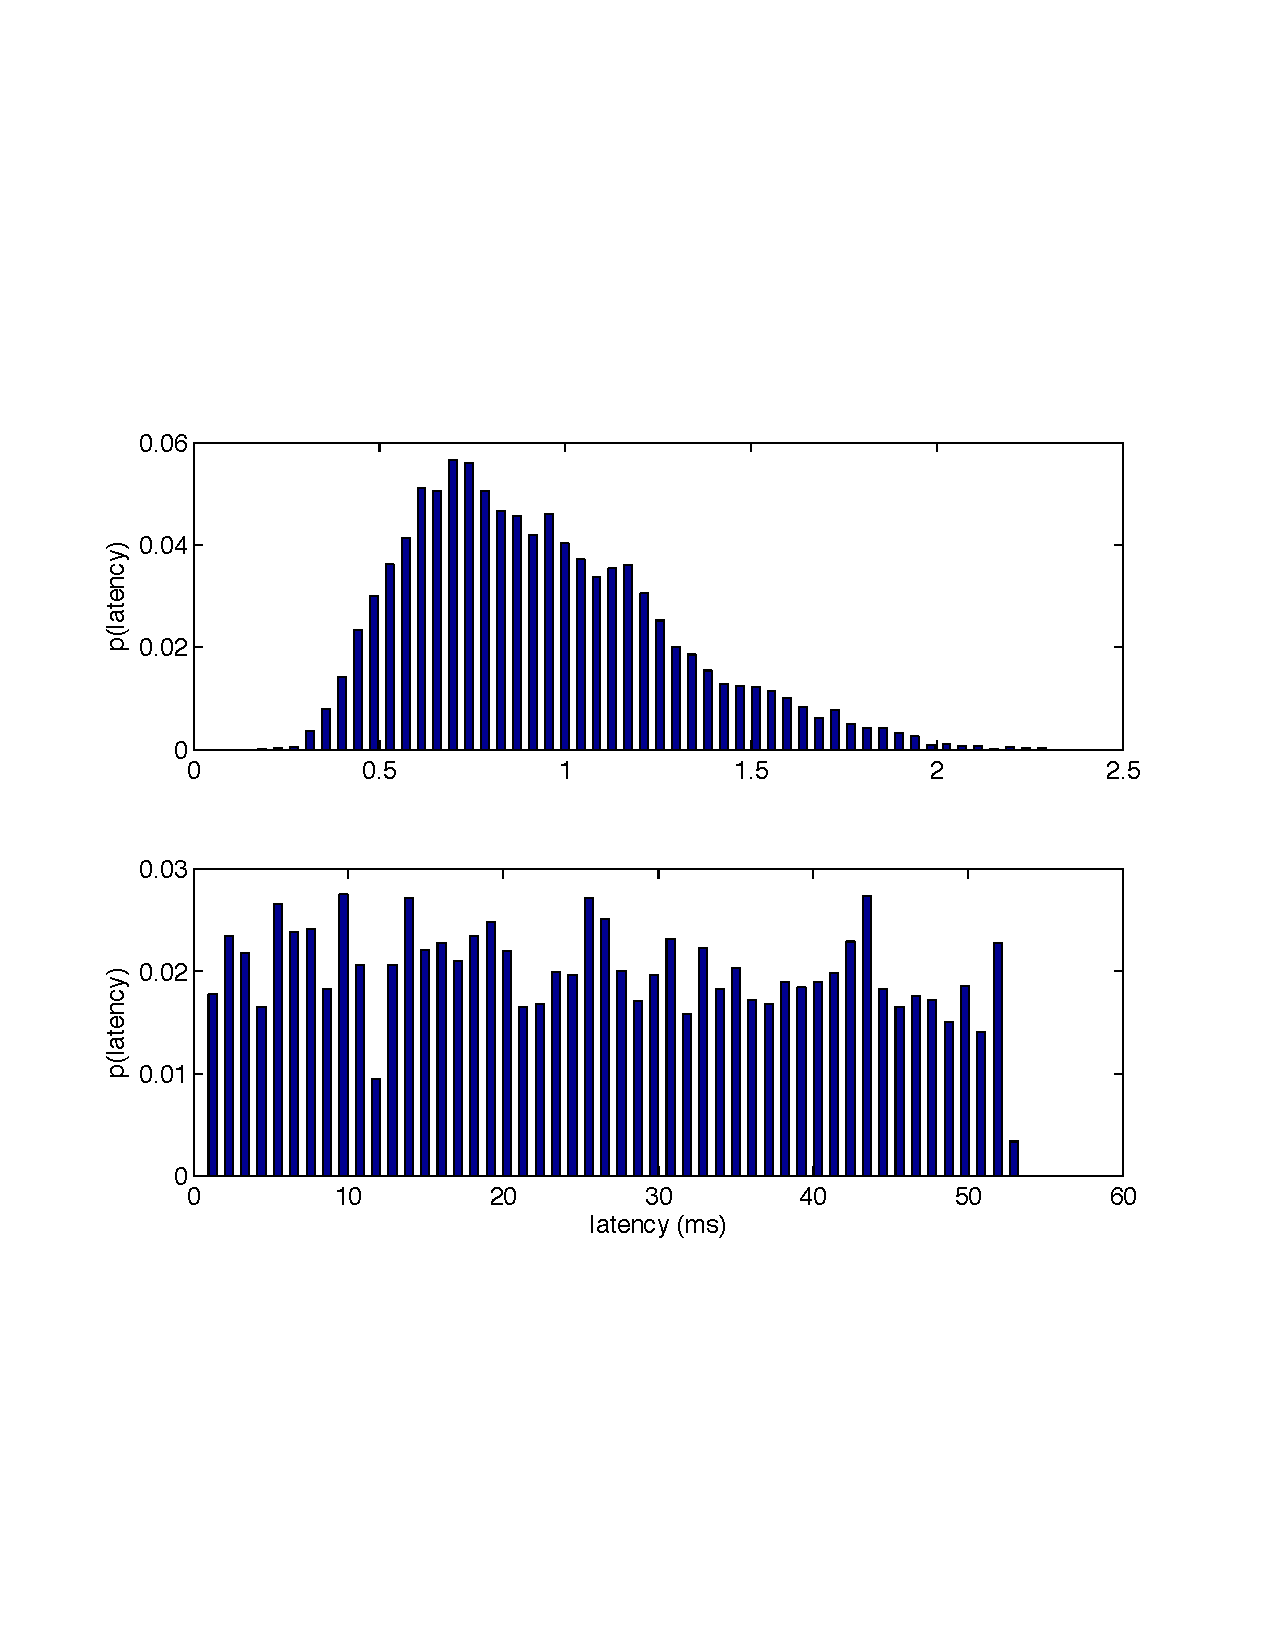
\includegraphics[width=0.45\columnwidth]{images/test_results/asynctest_50_clients_10k_20Hz}}\hfill{}\subfloat[Sending and receiving 100KB messages. ]{\centering{}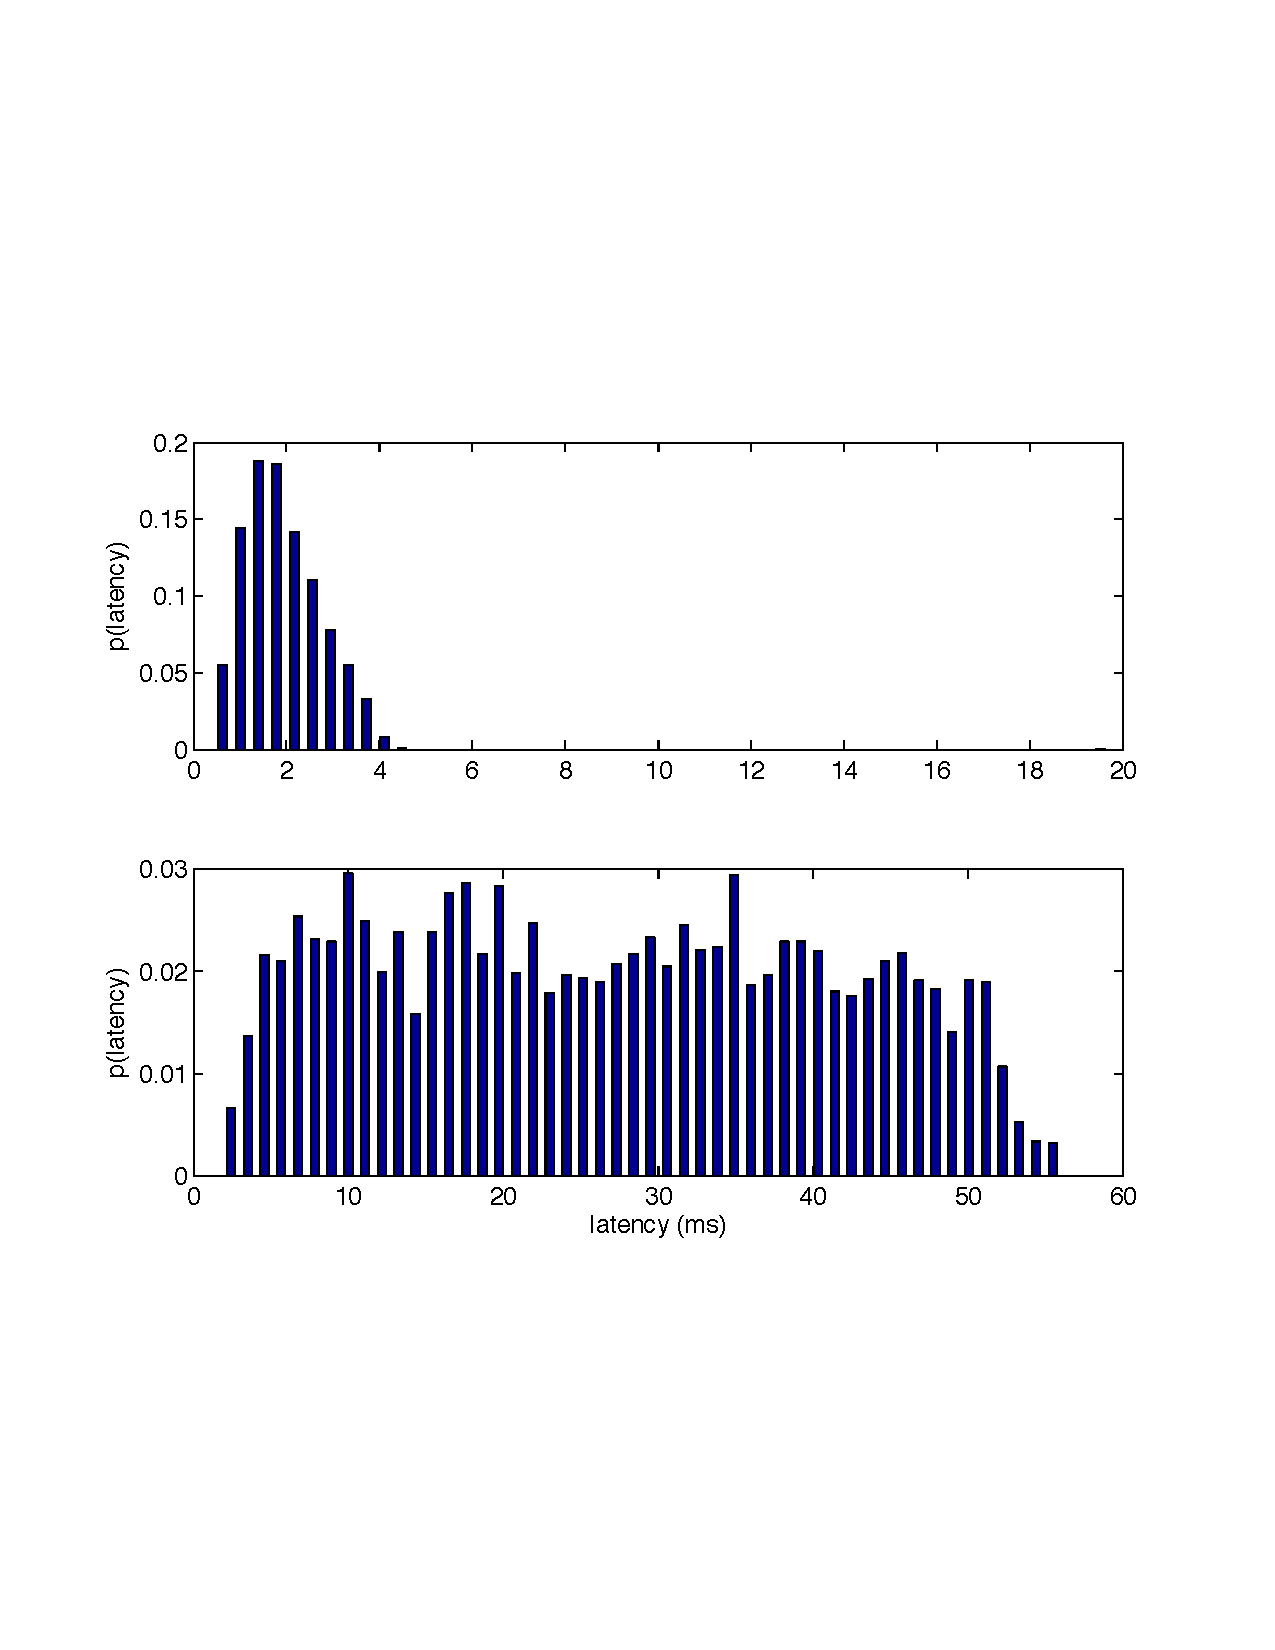
\includegraphics[width=0.45\columnwidth]{images/test_results/asynctest_50_clients_100k_20Hz}}\hfill{}\subfloat[Sending and receiving 1MB messages at 10Hz]{\centering{}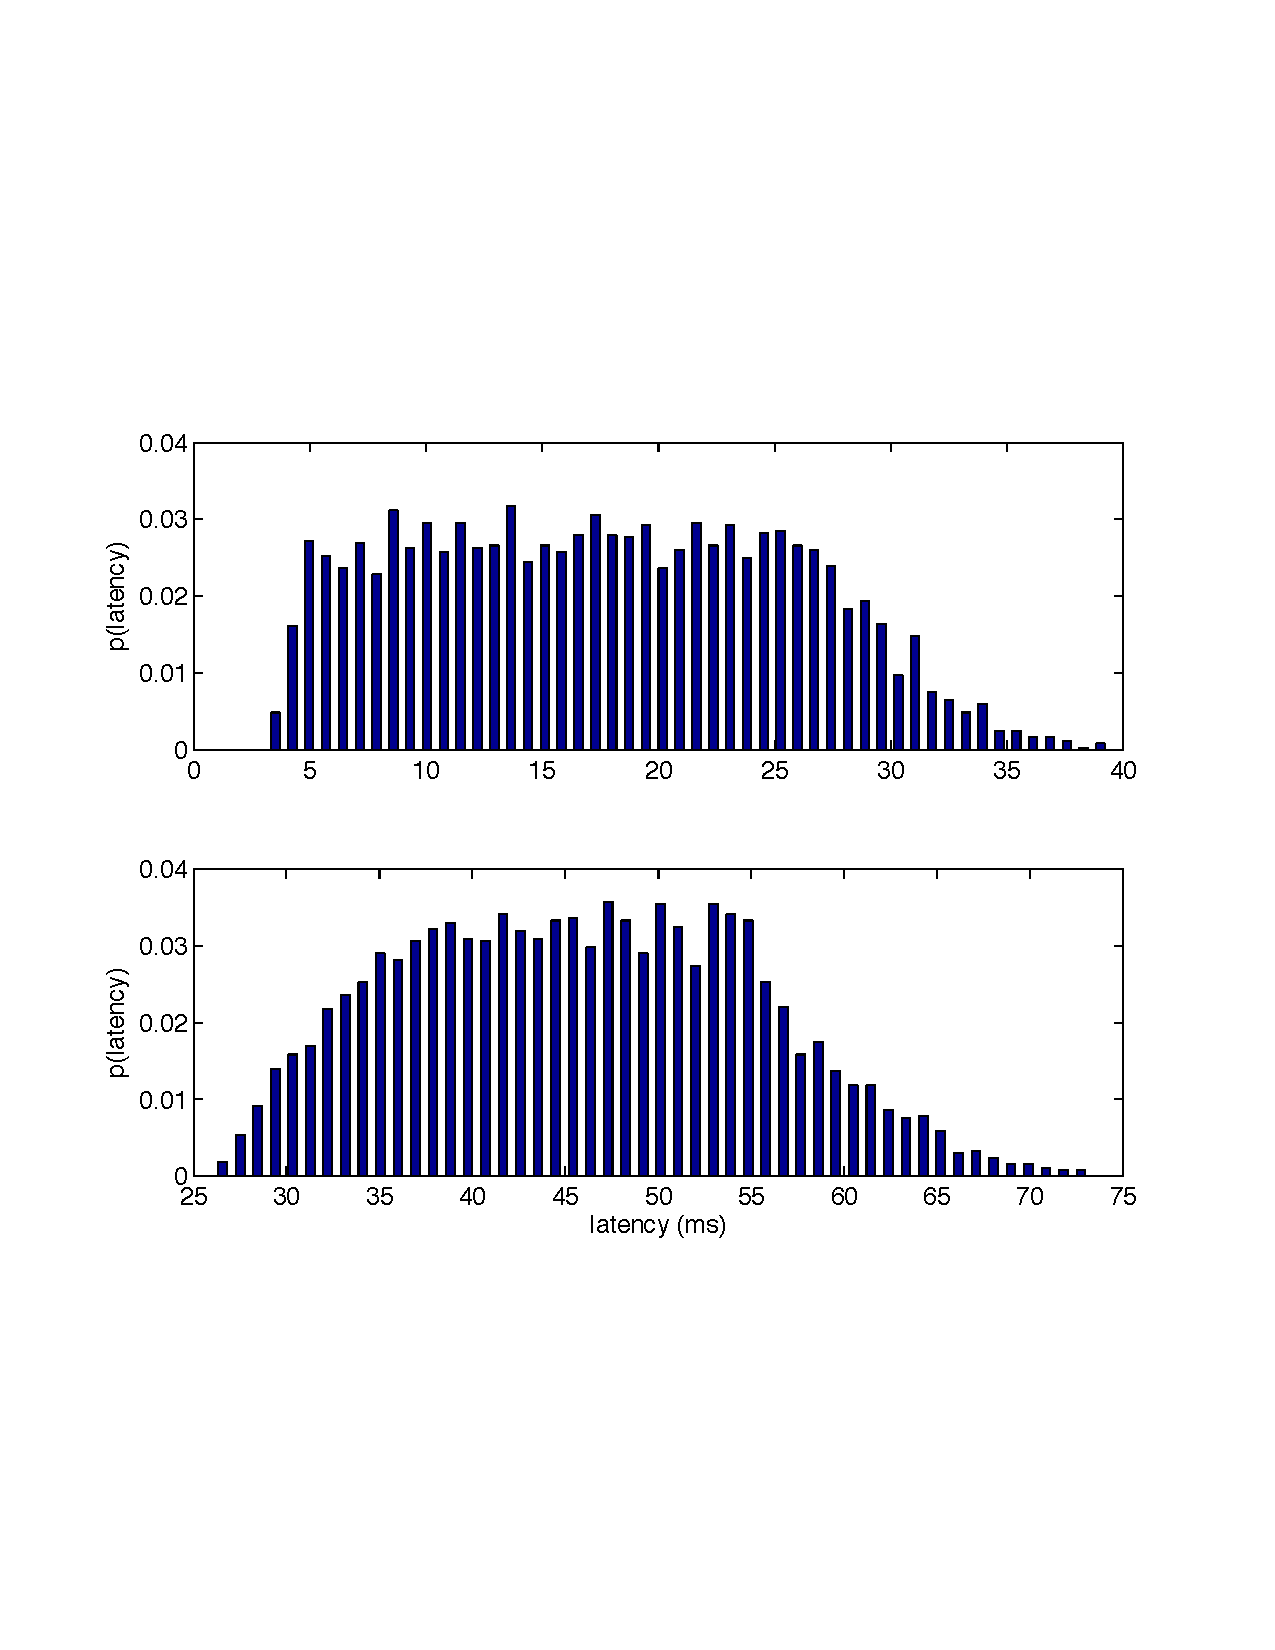
\includegraphics[width=0.45\columnwidth]{images/test_results/asynctest_50_clients_1M_10Hz}}\caption{Histograms of latencies between sending and receiving 1KB,10KB, 100KB
and 1MB messages. Messages are sent to 50 clients at 20Hz unless otherwise
stated. Top figures are for asynchronous clients lower figures are
for pre V10 clients with a comms-tick to 20Hz. All cases are suing
the \texttt{V10 MOOSDB. }As an example of total through put take the
example of sending 100KB messages to 50 clients 20 times a second
so 100K{*}50{*}20=100MB/s.}
\end{figure}

\par\end{center}

\clearpage{}


\section{Example Codes}


\subsection{The simplest example using \texttt{MOOSAsyncCommClient}}

The simplest (in terms of its proximity to the core communication
classes) example of using MOOS-V10 communications is given in figure
\ref{fig:The-simplest-example}. Here a MOOS::MOOSAsyncCommClient
is instantiated in its rawest form. It is configured with a Mail and
OnConnect callback and set free with a call to Run. Note that in the
Connect callback it registers for the data that is being posted once
a second in the main() forever loop. Many MOOS users will be used
to using CMOOSApp which manages the interaction with the Comms Client
Objects however it is instructive to look at the most fundamental
example. The CMakeLists.txt file for this example is also given below.

\lstinputlisting[caption={A simple example using MOOSAsyncCommClient}]{examples/CommsExample/CommsExample.cpp}

\lstinputlisting[caption={CMakeLists.txt to the simple example above}]{ examples/CommsExample/CMakeLists.txt }


\subsection{The Simplest Example using CMOOSApp}

We can of course achieve the same thing by subclassing CMOOSApp. The
code listing below shows how.

\lstinputlisting[caption={A simple example using MOOSAsyncCommClient}]{examples/AppExample/AppExample.cpp}


\subsection{Sharing Video Rate Data}

Here is a simple example code for sharing video data using the package
OpenCV %
\footnote{so you will need OpenCV installed on your machine. The CMakeLists.txt
file should find this installation and handle everything for you but
if you are using mac ports you may need to specify the location of
OpenCV in the ccmake gui as Cmake does not look in /opt by default. %
}. The program can be started in one of two ways - once as a server
which opens a camera and starts streaming images and as a client which
displays them in a window. Note this is not an elegant program - it
fixes the images size and does a fairly ugly bit of memory management.
It is presented here as a quick and dirty exposition of using MOOS
to send data at a moderate rate - its not an example of good use of
OpenCV. 
\begin{itemize}
\item Start a MOOSDB
\item To start a server in a terminal window from the command line whilst
in the directory containing the binary type :\texttt{ }

\begin{itemize}
\item \texttt{./camera\_example -s -{}-moos\_name SERVER}
\end{itemize}
\item To start a client from a similar terminal to that above type : 

\begin{itemize}
\item \texttt{./camera\_example -{}-moos\_name A}
\end{itemize}
\item To start another client, you guess it, open another terminal and try

\begin{itemize}
\item \texttt{./camera\_example -{}-moos\_name B}
\end{itemize}
\end{itemize}
If you do the above you should see you camera output appearing in
two windows with very little lag. 

\lstinputlisting[caption={Example code to build a camera sharing example}]{examples/VideoShare/CameraExample.cpp}

\lstinputlisting[caption={CMakeLists.txt to build the camera sharing example above}]{ examples/VideoShare/CMakeLists.txt }

There are several things to note about this example which are worth
spotting:
\begin{enumerate}
\item The way in which MOOS-V10 can handle command line argument parsing
for you using the \texttt{OnParseCommandLine()} virtual function in
\texttt{CMOOSApp}. Also note that the switches like \texttt{-{}-moos\_name}
are handled automatically for you. If this is a surprise read section
\ref{sub:Common-Command-Line}.
\item The way in which in this example \texttt{SetIterateMode} is used to
make the application respond quickly to the reception of mail.\end{enumerate}

\end{document}
